%\documentclass[a4paper, onecolumn, 12pt, doublespace]{article}
\documentclass[a4paper,onecolumn, 10.5pt]{article}
%\documentclass[a4paper, onecolumn, 11pt]{article}

%\usepackage[top=1in, bottom=1.25in, left=1.25in, right=1.25in]{geometry}
\usepackage{geometry}
\geometry{
	letterpaper,
	total={165.1mm,228.6mm},
	left=24mm,
	top=24mm,
}

\usepackage{amssymb}
\usepackage{amsmath}
\usepackage{bm}% bold math
\usepackage{bbm}
%\usepackage{biblatex}
%\usepackage[backend=bibtex]{biblatex}
%\usepackage[numbers,sort&compress]{natbib} % bibliography style
\usepackage[numbers]{natbib} % bibliography style
\usepackage[pdftex,bookmarks=true,bookmarksnumbered=true,plainpages=false,pdfpagelabels, colorlinks=true,
linkcolor=darkgray,
urlcolor=darkgray,
citecolor=gray]{hyperref}
\usepackage{url}
\usepackage{units}
\usepackage{doi}
\usepackage{graphicx}
\usepackage{dcolumn} % Align table columns on decimal point
\usepackage{listings} % To show code in part of the pdf
\usepackage{color}
\usepackage{authblk}
%\usepackage[nottoc]{tocbibind}
%\usepackage{notoccite}% PREVENTS CITES IN CAPTIONS FROM MISNUMBERING YOUR REFERENCES
\usepackage{setspace}
\usepackage{float}
\usepackage{multicol}
\usepackage{parskip}% http://ctan.org/pkg/parskip
\usepackage[utf8]{inputenc}
\usepackage[font=scriptsize]{caption}
\usepackage{tikz,lipsum,lmodern}
\usepackage[most]{tcolorbox}
%%\usepackage{LuaTeX}

\definecolor{mygray}{rgb}{0.90,0.90,0.90}
\definecolor{darkgray}{rgb}{0.33, 0.33, 0.33}


\title{%
	\textbf{appreciate} \\
	\large Digital Ownership Enabled Utility  \\
	\scriptsize v0.9.7
}
\author{\scriptsize{ Jeremy McEntire, Moriah Waterland, Kayla Trivieri, Z Braithwaite, Devon Stewart,  Allys Ton, Justin Connor }}
\date{\normalsize{October 31, 2022}}

\begin{document}
	%\setlength{\parindent}{0pt}
	
	\maketitle
	
	
	\begin{tcolorbox}[colback=gray!0!white,colframe=gray!0!white, boxed title style={empty, size=minimal, bottom=1.5mm}]
		  
		
			\abstract{appreciate is building a digital Proof of Ownership ecosystem. Our platform ingests moments of Item purchase, in the form of transaction receipts, and creates Proof of Purchase (PoP) Credentials. PoP Credentials are Verifiable Credentials (VCs) that digitally link Item and Owner using the Owner’s Decentralized Identifier (DiD). PoP Credentials establish the Item’s chain of custody and absorb Item use metadata. These interactions exist as primitives in the appreciate ecosystem, a secure-by-design architecture which iterates on conventional Service Oriented Architecture (SOA) solutions by hosting logic inside a controlled environment rich with data and other constructs. The ecosystem is constructed such that partners can focus on delivering utility services to Owners. Proof of Ownership (POwn), our core primitive, is only required when an Owner requests access to a service. In fact, service providers may embed Proof of Ownership requirements directly in their services. To access services, Owners action a PoP to ‘confirm’ POwn. This confirmation comes in the form of a McEntire Score (M Score): a proprietary assessment of factors to determine appreciate’s confidence in a PoP holder’s possession of the associated Item. PoP and M Score define whether POwn is confirmed or requires more evidence.  As the ecosystem expands, we intend to capture PoP and M Score as on-chain Item Tokens (dynamic NFTs) and to enable commerce denominated in the appreciate fungible token.  appreciate has no consumers or users, only Owners. We look forward to contributing to the Owner Economy.
		}
	\end{tcolorbox}
	
\newpage
\tableofcontents
\newpage
	
\setlength{\parindent}{0em}
\setlength{\parskip}{8pt}
	%\doublespacing
\section {Introduction}


	300 billion receipts per year -- humanity tracks our Item transactions through this mess of plastic, paper, and server space.  Each time an Item is transferred to an Owner, we humans generate unnecessary waste (annually 4 billion pounds of $CO_2 $ and 302 million pounds of solid waste\cite{envimp}). In addition to their wastefulness, receipts are analog in a digital world. They don’t enable digital ownership: no chain of custody, and no Item-related utility.
	

Item related utility, the ability to do stuff with stuff, is a hard problem to solve. Enabling Item related utility requires an ecosystem with the following elements:
\begin{enumerate}
	\item Digital chain of custody for each Item
	\item Methods to link physical Items to their digital counterparts
	\item Ability for organizations to easily offer integrated services
	\item An application layer through which Owners access services
\end{enumerate}

Each of these features is complex, and each is not valuable without the others. When building an ecosystem to solve the Item related utility problem, we considered one principle as paramount: seamlessness. Without automated onboarding and simple utility, Owners would not enter the ecosystem, let alone take action in it. Deciding on receipts as our input guarantees scale. Automated ingestion of receipts make it easy for Owners to engage with appreciate, and immediate utility increases the value of their engagement. All of this is our effort to create a new Owner Economy, powered by Extensible Ownership.

The appreciate team is obsessed with Extensible Ownership: physical Items enhanced with chains of custody and/or digital twins. Extensible Ownership enables seamless utility -- doing stuff with stuff. 
Currently, humans do plenty of stuff with stuff: we finance it, insure it, resell it, customize it. 
Yet, this utility is far from seamless, often siloed, and is only a small sample of the utility enabled by Extensible Ownership. 

Empowering Owners in a secured and trusted manner is at the core of our values. The appreciate ecosystem addresses the three fundamental principles in cybersecurity, known as the CIA triad: confidentiality, integrity, and availability. 
Traditional Web1/Web2 products are rarely able to address all three, creating vulnerabilities and exposing users to potential risk. 
appreciate’s design solves this problem using a data transport structure (cryptogram) that optimizes CIA control settings at each point of transit, computation, or storage. 
The secure-by-design approach facilitates integrations with partners making data available for delivering Owner utility. 

Our approach to security, human-centered design, and interoperability redefines the membrane between all digital and physical items, transforming the ownership experience (See \(Fig.~\ref{fig: flowchart}\)).
appreciate is the future of Ownership.  



\begin{figure*}[!htb]
	\centering %trim=left botm right top
	%\fbox{
		\includegraphics[clip, trim=0cm 2cm 0cm 7.5cm, width=0.80\textwidth]{./images/flowchart.pdf}
		%	}
	\caption{From Receipt Ingestion to Extensible Ownership and Utility  }
	\label{fig: flowchart}
\end{figure*}



\section {appreciate Concepts}

\begin{tcolorbox}[colback=gray!5!white,colframe=gray!50!black, title=appreciate experience for Item Owners]	
	appreciate is a space for Owners to confidently track, manage, and unlock utility associated with their possessions.  Receipts ingested by the appreciate ecosystem are parsed and issued as Proof of Purchase Credentials.  Owners can manage their collection of PoP Credentials (as Items) in their appreciate wallets. These credentials can unlock experiences within the ecosystem; such as airdrops, invitations, and third-party service offerings. 
\end{tcolorbox}


Security and privacy considerations influenced the design and development of the ecosystem creating an architecture that is secure by default. End-to-end encrypted communication enables Owner-managed privacy allowing Owners retain control of both the Items in their wallets and their personal data.
Additionally, the ecosystem is interoperable and extensible. The integration portal allows services to easily and securely connect with our ecosystem without the need for an independent integration team or additional resources. Traditional approaches to integration require onerous integration processes dealing with third-party services, networking, and other constraints. The ecosystem hosts and executes business logic for third parties, providing privileged access to secure information and low-latency interactions. Furthermore, the ecosystem simplifies access to integrated services such as post-purchase experiences, P2P interactions, or blockchain on-ramps. 

\begin{figure*}[!htb]
	\centering %trim=left botm right top
	%\fbox{
		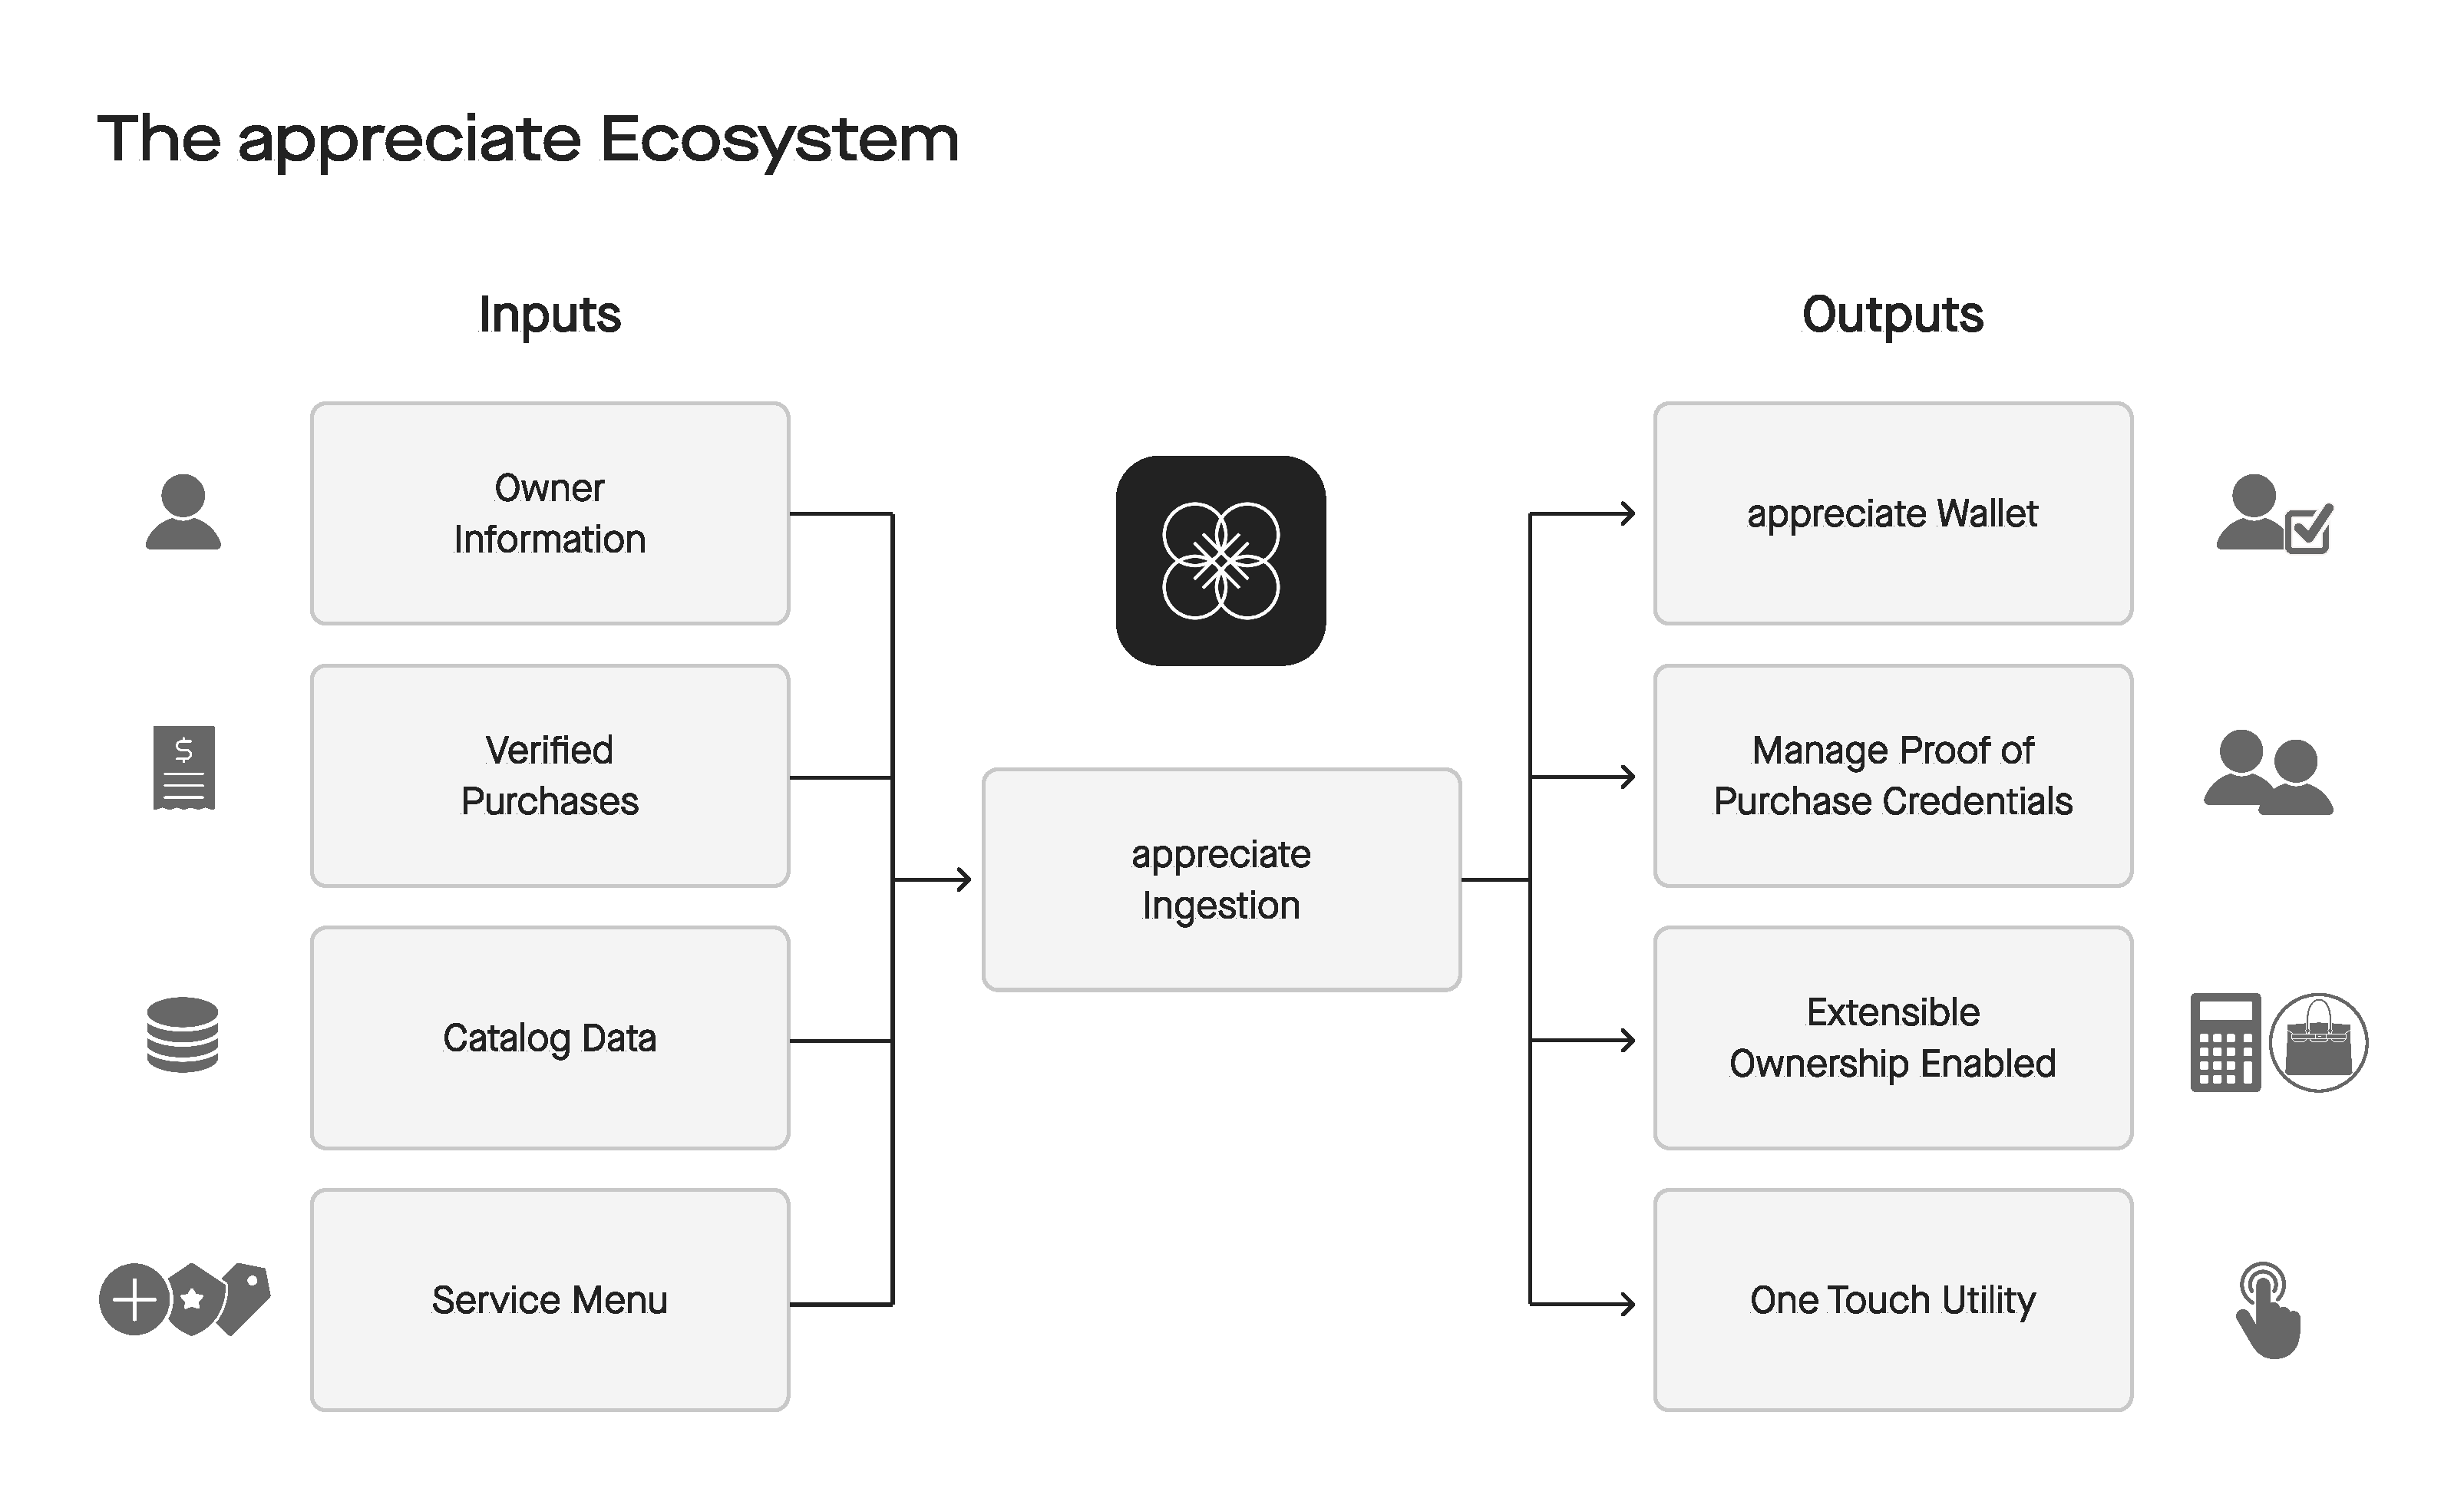
\includegraphics[clip, trim=0cm 2cm 0cm 6cm, width=0.80\textwidth]{./images/Ecosystem.pdf}
		%	}
	\caption{The appreciate Ecosystem }
	\label{fig: ecosystem}
\end{figure*}



\subsection{Proof of Purchase}

Proof of Purchase Credentials are automatically created from receipts gathered by the platform in one of the following ways:
\begin{enumerate}
	\item \textbf{Direct Integration} - The platform is integrated with partner APIs and point of sale systems. 
	\item \textbf{Receipt Uploading} - Owners can upload receipt images for an Item via the appreciate app. The receipt is validated and the PoP in the Owner’s wallet is verified.
	\item \textbf{Receipt Forwarding} - Owners can forward receipts from partner brands to send@appreciate.it. The receipt is parsed and PoPs are automatically populated into Owner’s wallets.
\end{enumerate}

Proof of Purchase takes the form of a verifiable credential (VC)\cite{verifiablecred}. A VC consists of a trust root that attests a fact about a certain actor at a specific point in time. 

\hspace{1cm} {\scriptsize Example: Brand A attests that Owner B purchased Item \#12345 at 12:56PM on 09/06/22 (for \$1000). }


\subsection {McEntire Score}

The McEntire Score is a value calculated in real time to determine appreciate’s level of confidence that a specific physical Item is possessed by the holder of the associated PoP (Owned).  Therefore, appreciate’s Proof of Ownership is a dynamic assessment, rather than an object itself.  The M Score is a compilation of supportive data lending credence to the claim that a specific Item is possessed by a PoP holder.

Considerations may include the length of the Item’s chain of custody, the amount of time since the Owner purchased the Item or last verified possession, the Items collected by the Owner, and the Owner’s activity related to the Item. The confidence score also takes into account the Owner’s identity, age of account, proof of purchase type, and Item details (e.g., serial number, NFC tags, etc).

Owners can bolster their M Score by taking certain actions within the ecosystem.
Examples of relevant actions:
\begin{enumerate}
	\setlength{\itemsep}{0pt}
	\item An Owner photographing the Item as a touchpoint for fingerprinting (see below)
	\item  A brand reporting that an Owner sent the Item in for repair
	\item If the Item has Near-Field Communication (NFC), the Owner’s phone shows the NFC signature
	\item An Owner sends an Item to an appreciate Vault for storage
\end{enumerate}



\begin{tcolorbox}[colback=gray!5!white,colframe=gray!50!black, title=M score components: item fingerprinting]

appreciate connects physical Items with their PoP Credential through the process we call fingerprinting – a technique similar to biometric fingerprint recognition, which builds a model identifying key features of an Item for later comparison. Other techniques, like NFC/RFID tagging, often require modifications to the Items or even changes in the manufacturing process. However, by utilizing high-quality images and advances in computer vision and machine learning, appreciate’s fingerprinting technology assesses the nuanced differences between Items to build compelling attestation in support of Proof of Ownership.\\
\newline
Damage or changes to Item landmarks may reduce the model’s accuracy, as with biometric fingerprinting. To minimize this impact, our models rely on a variety of features rather than just a few. Additionally, the models are updated with new data when fingerprinting is confirmed, generating a new posterior which accommodates for the natural aging of Items.\\
\newline
The appreciate fingerprinting solution trained a convolutional neural network (CNN) variant to learn the features that distinguish one Item instance from another—the model does not care that any two macroscopic features are similar to one another. It has been asked to learn what makes Items different from one another on a more nuanced level. When the trained model is shown a new image, it is asked to detect every recognizable feature. Of course, each image presented to the model may include only one of the identified features, so a set of images are presented from various angles to ensure the model can remain accurate even when the Item inevitably changes over time.
\end{tcolorbox}



\subsection {Proof of Ownership}

appreciate’s ultimate goal is to establish Proof of Ownership -- a concept that represents the level of entanglement between the physical Item and its PoP Credential.  We represent Proof of Ownership indirectly in the form of a PoP Credential with an associated M Score. Essentially, this PoP Credential is a record locator, the control of which can be proven by the Owner.

The Proof of Ownership allows appreciate to convincingly demonstrate that the person who controls the PoP Credential is the same individual who possesses the associated physical Item.  Proof of Ownership is confirmed/denied at the moment a service is requested.  This confirmation is based on the service provider’s requirements.  For example, to offer Item Insurance in the appreciate ecosystem: Insurance Provider A may require a PoP and M Score $>50$ to ‘confirm’ ownership, Insurance Provider B may require a PoP and M Score $>65$ to ‘confirm’ ownership.  

\begin{tcolorbox}[colback=gray!5!white,colframe=gray!50!black, title=A case for Proof of Ownership: Item Insurance 
	]
	
	Lacking reliable means to prove ownership of an Item decreases the total market for Item insurance, impairing both insurance companies and Item Owners. Building on appreciate, a third party Insurance provider can access real time Proof of Ownership confidence scores with which to make coverage decisions. Proof of Ownership increases the total addressable market for insurers, overall insurability of each Item. This in turn decreases the costs associated with coverage, enabling benefits for both insurer and Owner.
	
\end{tcolorbox}

In the future, Owners may request an on-chain Item Token to represent their Item.  This Item Token will be minted as a dynamic NFT - representing the Item, but also the M Score of Item-Owner entanglement.  We contemplate that any Item Token may be decoupled from the physical Item.  In the case of this decoupling; the Item Token holder may benefit from digital experiences associated with the Item Token, while the Item Owner may relinquish access to some services requiring digital Proof of Ownership.

See \(Fig.~\ref{fig: poptpoo}\) for Proof of Purchase to Proof of Ownership workflow

\begin{figure*}[!htb]
	\centering %trim=left botm right top
	%\fbox{
		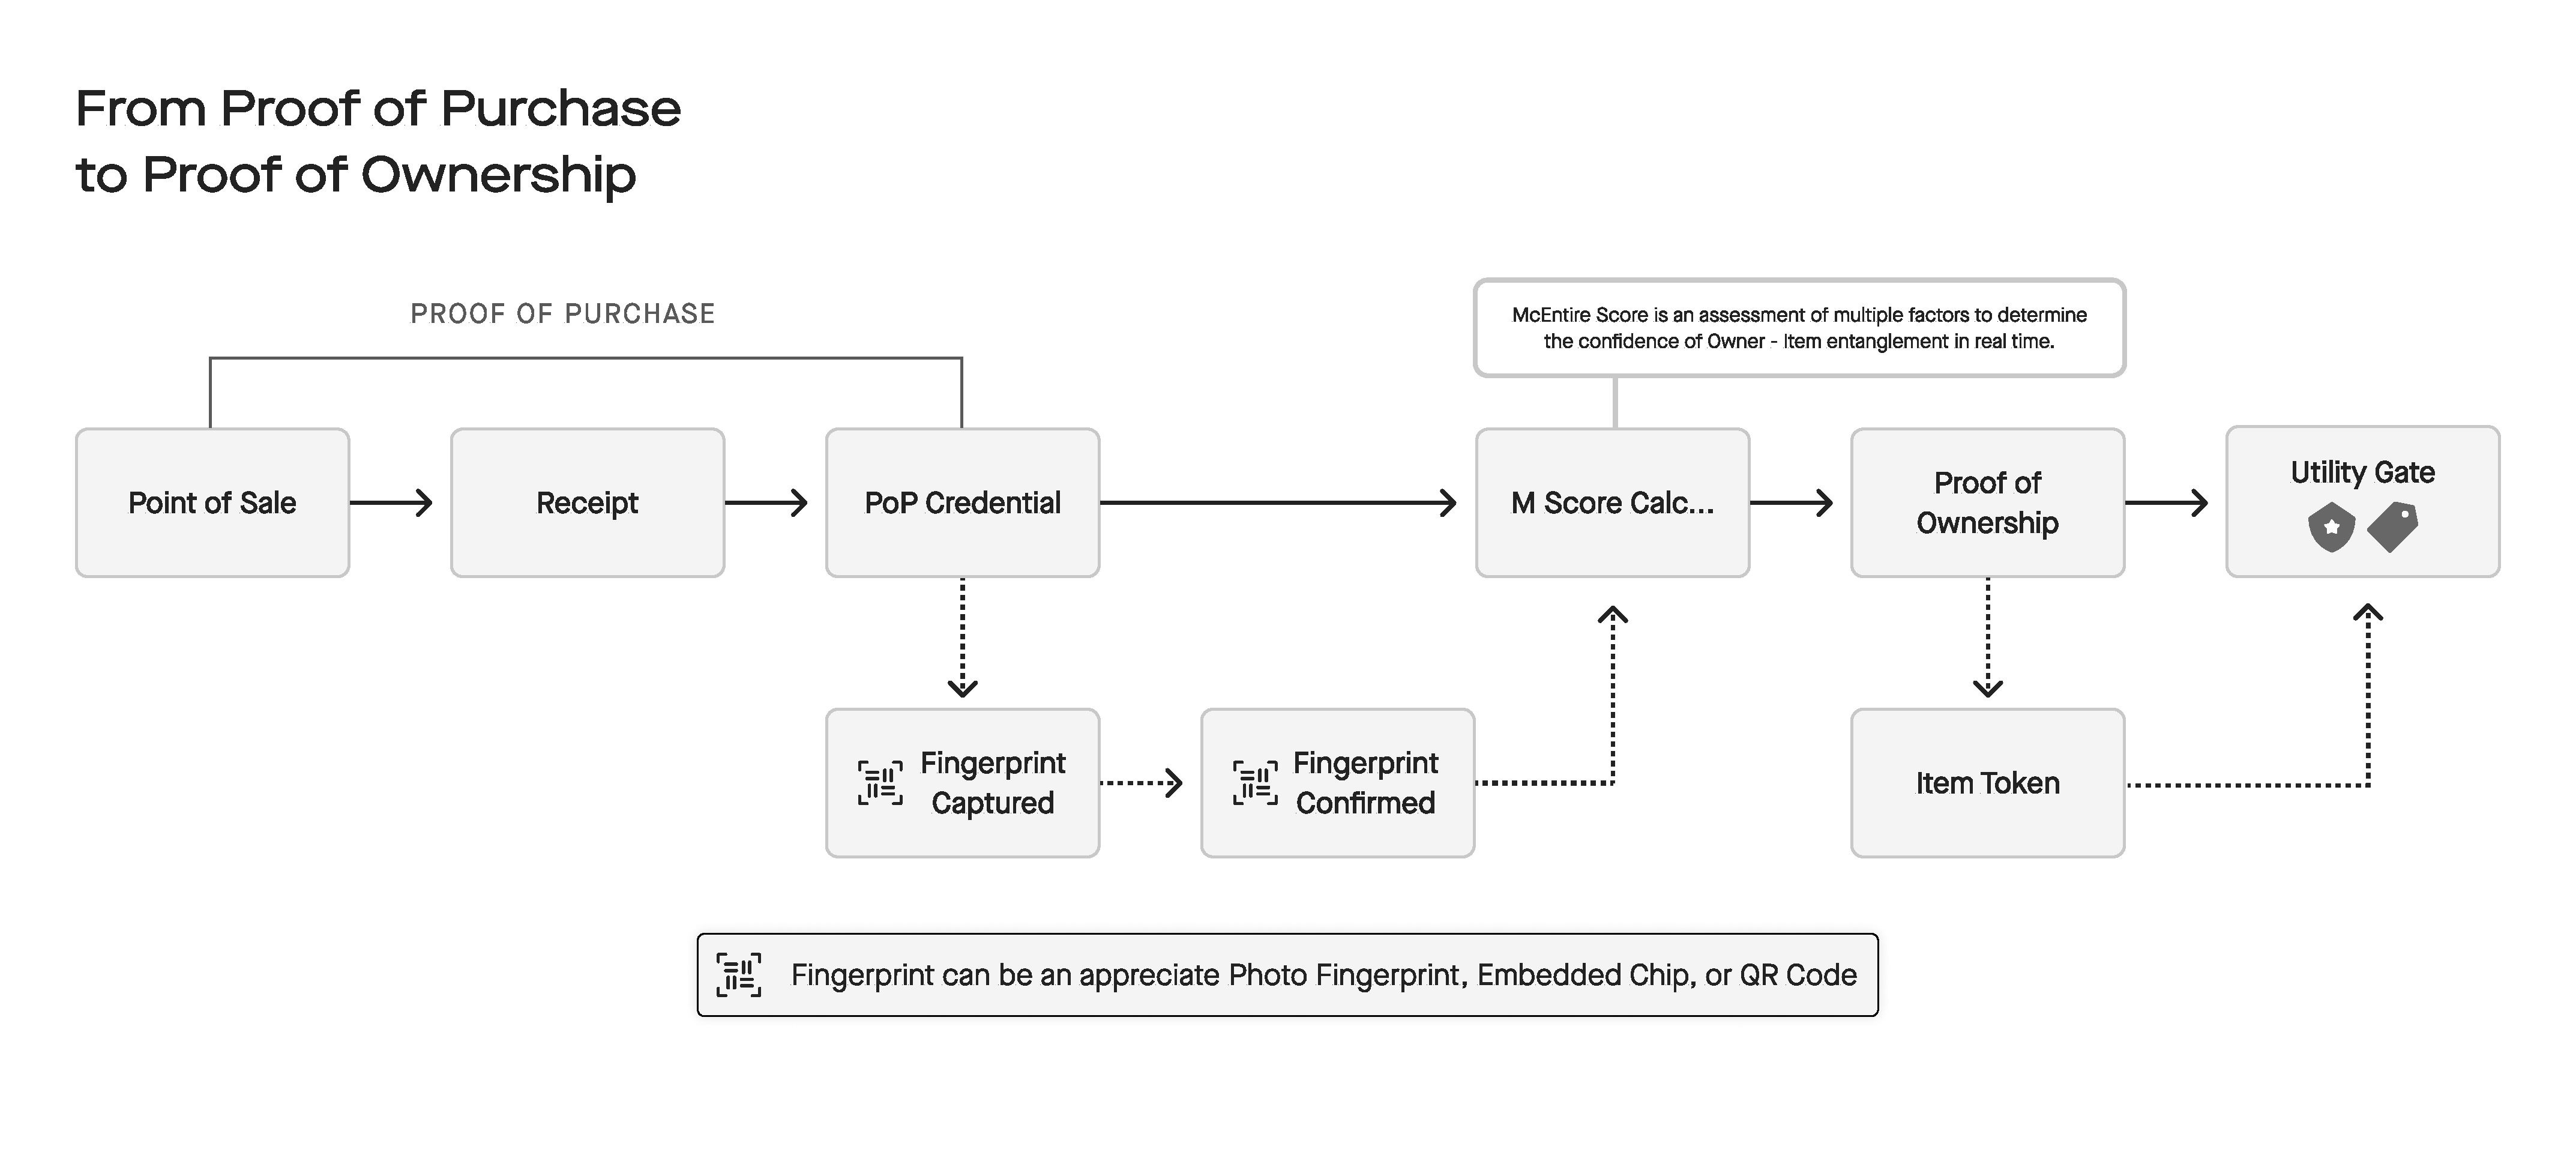
\includegraphics[clip, trim=0cm 2cm 0cm 6cm, width=0.80\textwidth]{./images/From_Proof_of_Purchase_to_Proof_of_Ownership.pdf}
		%}
	\caption{From Proof of Purchase to Proof of Ownership }
	\label{fig: poptpoo}
\end{figure*}




\section{appreciate Architecture}

\subsection{Design Considerations}
Leading industry practices utilize disparate solutions for addressing challenges in the information security triad (CIA: confidentiality, integrity, and availability) but lack comprehensive solutions that allow discrete calibration of the individual elements. Current solutions should also accommodate Zooko’s trilemma\cite{zooko} including namespaces that are Human-Meaningful, Secure, and Decentralized.

The appreciate ecosystem is an adaptive, automatically-scalable architecture that invokes and calibrates platform controls for support in accordance with service needs in availability, integrity, and confidentiality. In a single system, appreciate addresses all three pillars of the Zooko Wilcox-O'Hearn conjecture through:


\begin{itemize}
	\item Decentralization - the appreciate ecosystem allows for replication by scaling horizontally as a stateless system balanced with DNS.
	\item Security - the layered, end-to-end encryption model starts with client-side encryption of each datum included in the request. This enables element-level disclosure via layered key sharing so that services process only the required data.
	\item Human-Meaningful - Our ecosystem utilizes abstractions to translate between human meaningful data and system-oriented data.	
\end{itemize}

By employing a secure-by-design strategy, appreciate adopts encryption by default for all actions and data. Our data transport structure -- colloquially referred to as a cryptogram -- optimizes confidentiality, integrity, and availability control settings at each point of transit, compute, or storage. Data is encrypted at all times except when strictly required for data transformation operations (e.g., read, write, modify).


\subsection{Availability}
appreciate’s ecosystem ensures the high availability and fault tolerance to provide business continuity of mission-critical applications and systems. As a result, high availability is achieved, targeting 99.999\% uptime and performing at the caliber of what is normally only possible by employing full-time SREs.

To achieve such high availability, the appreciate ecosystem follows a distributed design. This allows the ecosystem to be deployed in any region, cloud, or data center independently, creating opportunities for redundancy and ensuring availability.

The appreciate ecosystem facilitates sending state updates to the requesting client so that interrupted or failed requests can be recovered and replayed beginning after the most recent successful state change. In the instance that an ecosystem component experiences an anomaly, any interrupted requests can be replayed, ensuring idempotency.

\subsection{Integrity}

The appreciate ecosystem follows the Biba Integrity\cite{biba} model. The simple integrity axiom restricts entities from reading any content created at a lower integrity level and the star integrity axiom restricts any entity from writing to a higher integrity level (See \(Fig.~\ref{bibamod}\)).

\begin{figure*}[!htb]
	\centering %trim=left botm right top
	\fbox{
		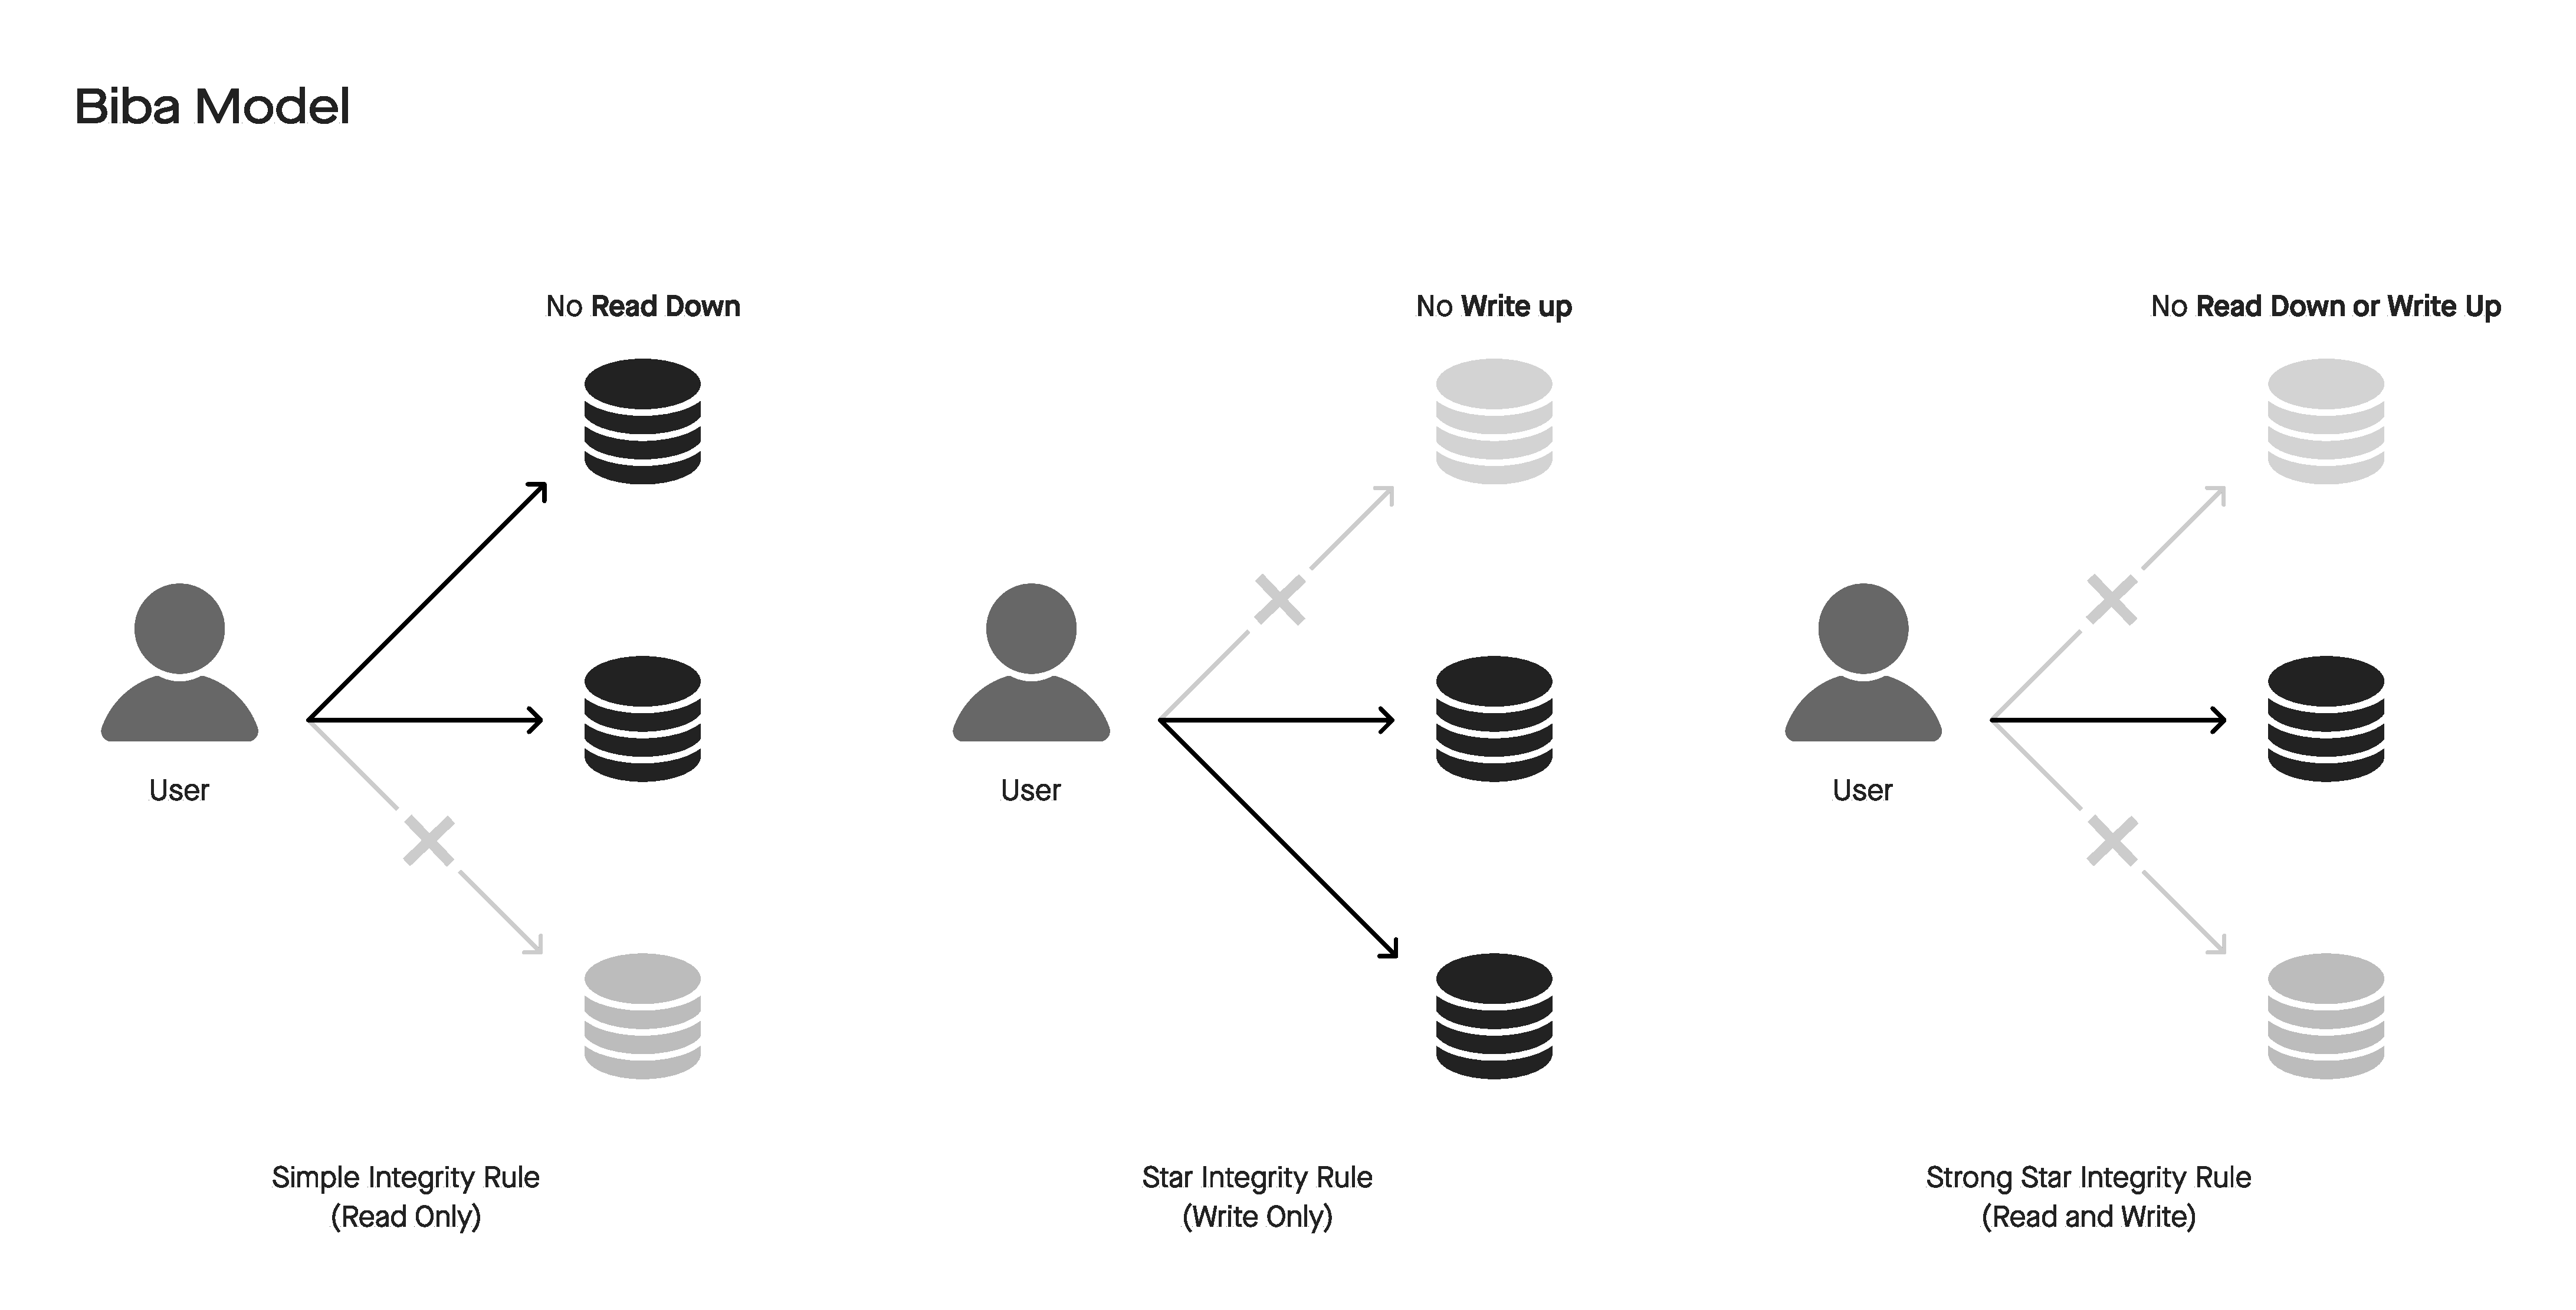
\includegraphics[clip, trim=0cm 2cm 0cm 6cm, width=0.80\textwidth]{./images/Biba_Model.pdf}
	}
	\caption{Biba Integrity Model}
	\label{bibamod}
\end{figure*}



Additionally, the ecosystem is interoperable and extensible. The integration portal allows services to easily and securely connect with our ecosystem without the need for an independent integration team or additional resources. Traditional approaches to integration require onerous integration processes dealing with third-party services, networking, and other constraints. The ecosystem hosts and executes business logic for third parties, providing privileged access to secure information and low-latency interactions. Furthermore, the ecosystem simplifies access to integrated services such as post-purchase experiences, P2P interactions, or blockchain on-ramps. 



\begin{figure*}[!htb]
\centering %trim=left botm right top
\fbox{
	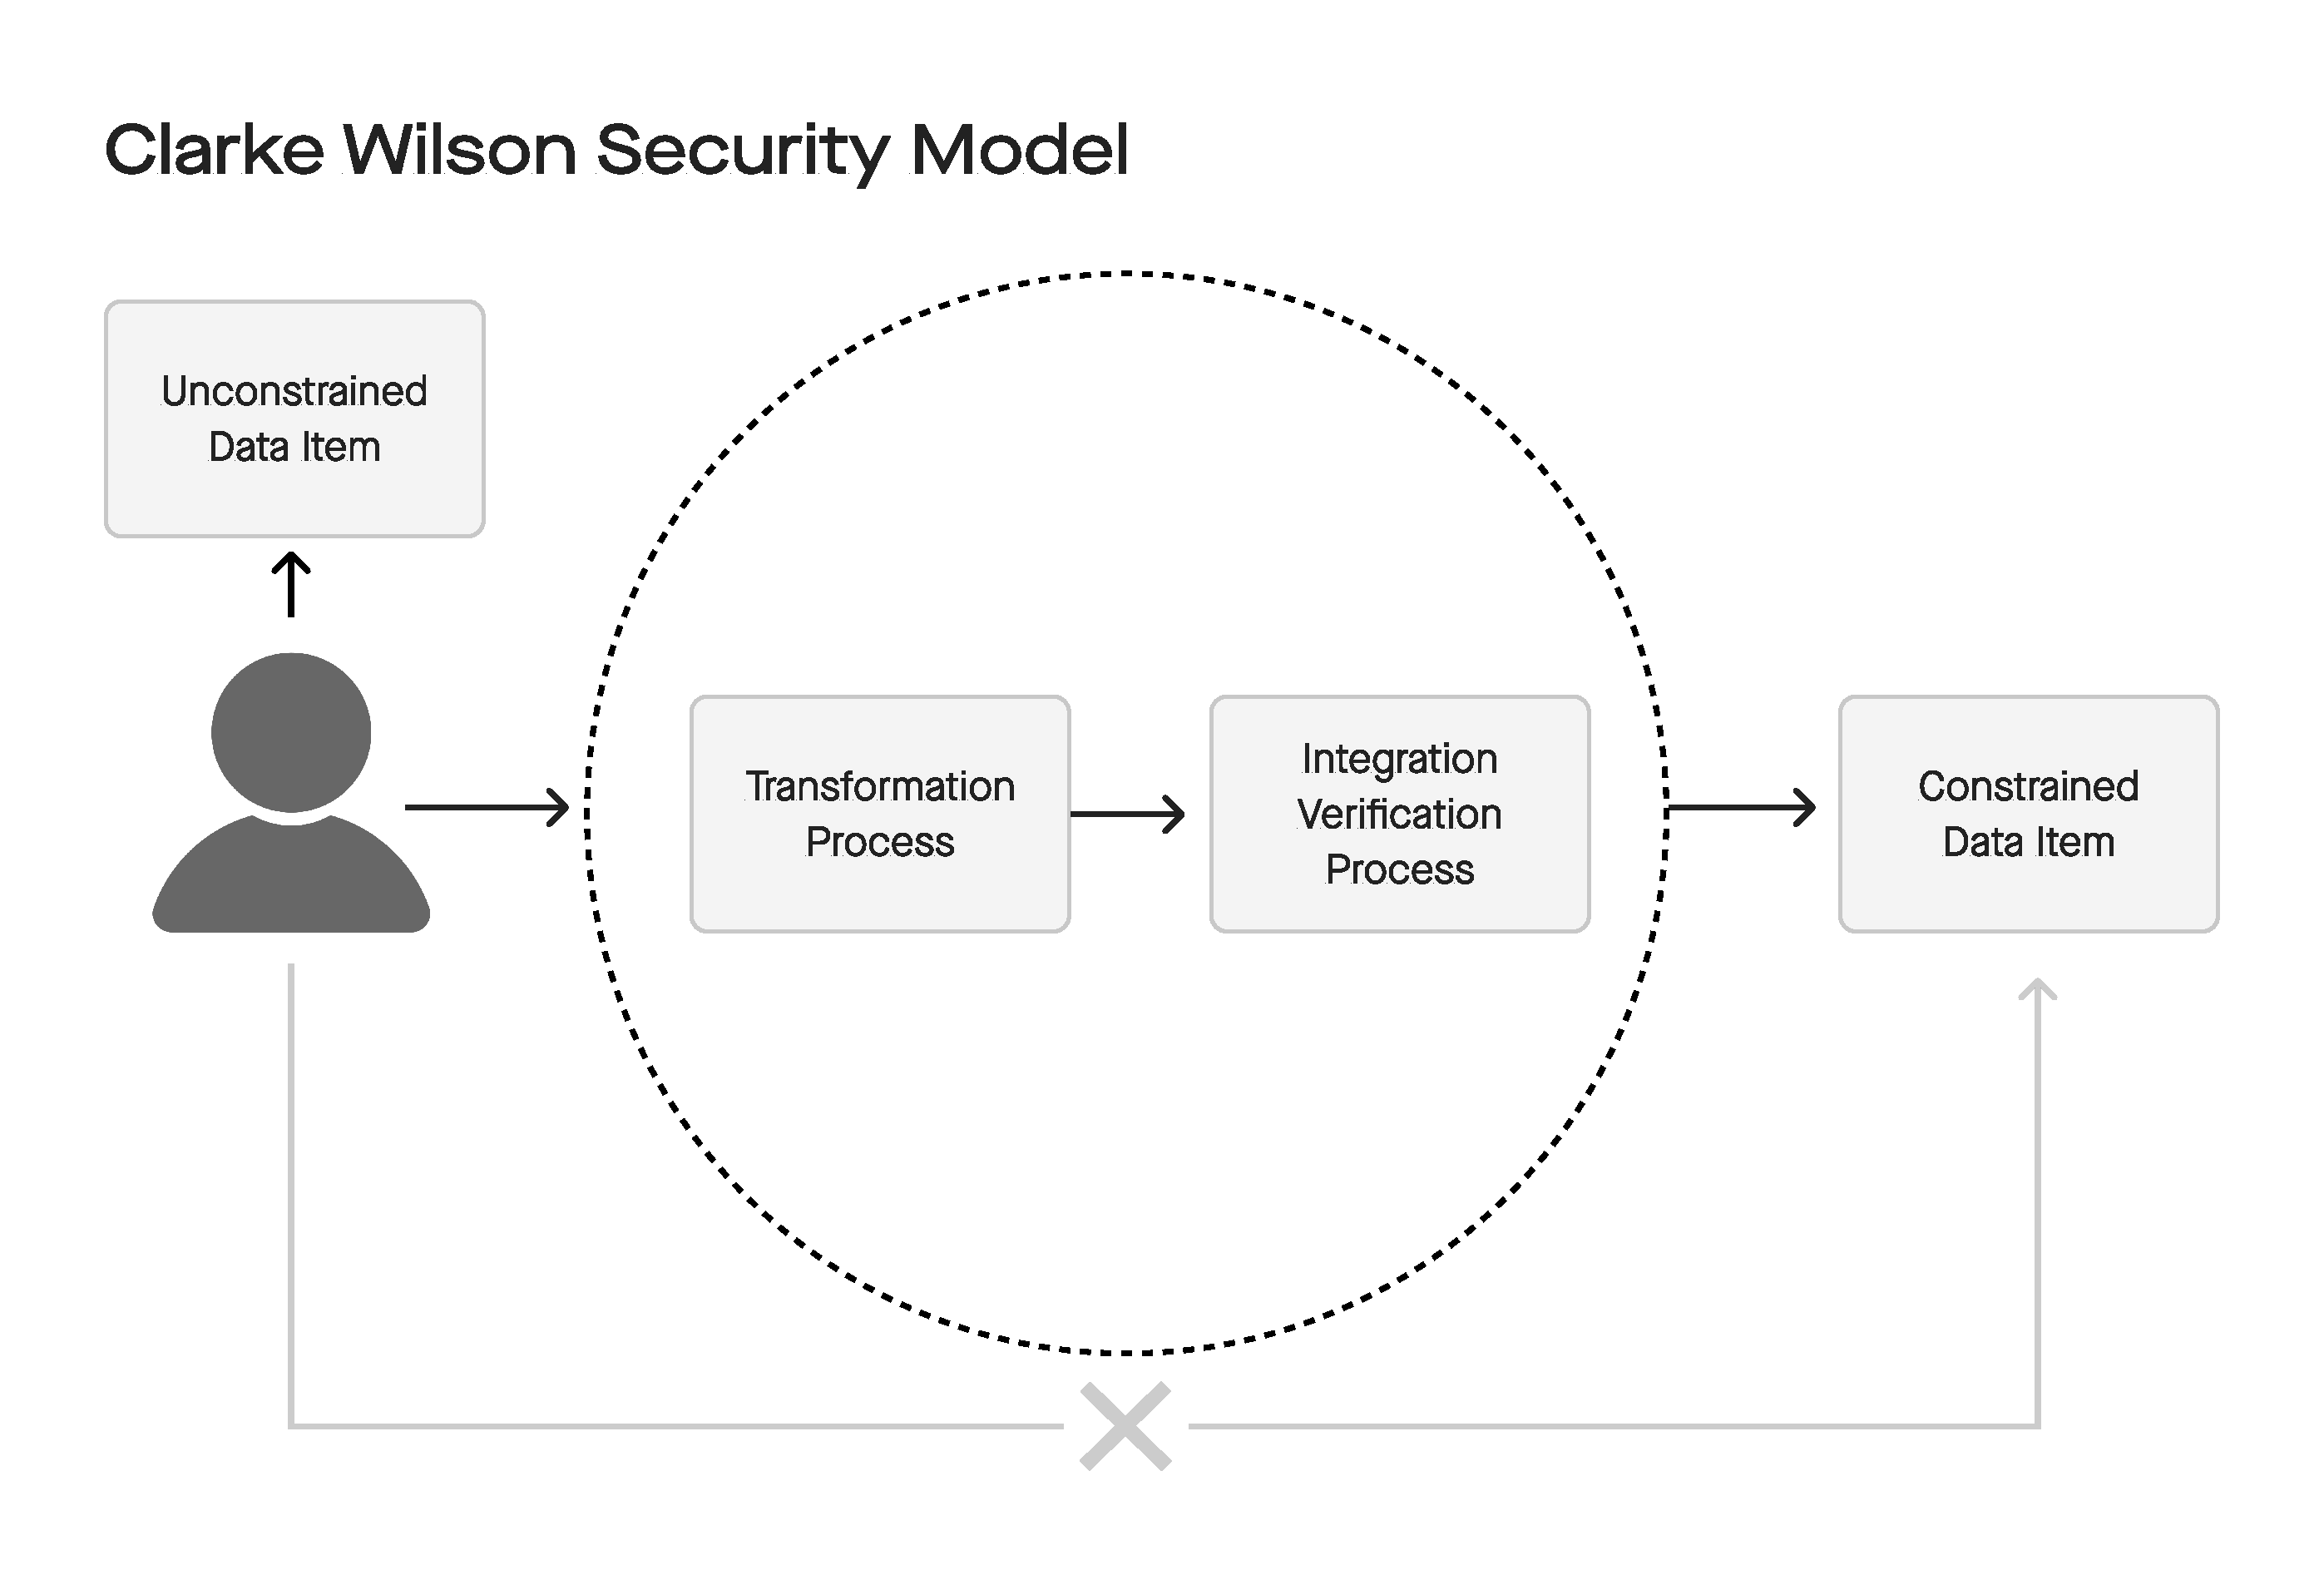
\includegraphics[clip, trim=0cm 2cm 0cm 5cm, width=0.80\textwidth]{./images/Security_model.pdf}
}
\caption{Clarke Wilson Security Model}
\label{fig: clarkwilson}
\end{figure*}


The appreciate ecosystem applies some level of restriction to all data elements in accordance with the Clark-Wilson model (See \(Fig.~\ref{fig: clarkwilson} \)). Constrained data Items must have integrity preserved and only allow modification for a transformation procedure. There are two main data classifications, restricted and unrestricted. Within the appreciate ecosystem, all data types are assigned some restriction level. Through applying data type parameters, we are able to lower the probability of fraud and abuse, and increase confidence and trust with our third party services. 


\subsection{Confidentiality}
The Bell-LaPadula (BLP)\cite{securecomp}model for data confidentiality restricts any entity from reading anything at any higher data classification than assigned, reversing the read-write conditions espoused by the Biba model (See \(Fig.~\ref{fig: bella} \)). 
 This is the simple security principle of this model. This model also restricts any entity from writing to a lower classification level. The most restrictive invocation of Bell-LaPadula is the strong star principle which restricts any entity from performing read or write functions to any level other than that assigned.

\begin{figure*}[!htb]
	\centering %trim=left botm right top
	\fbox{
		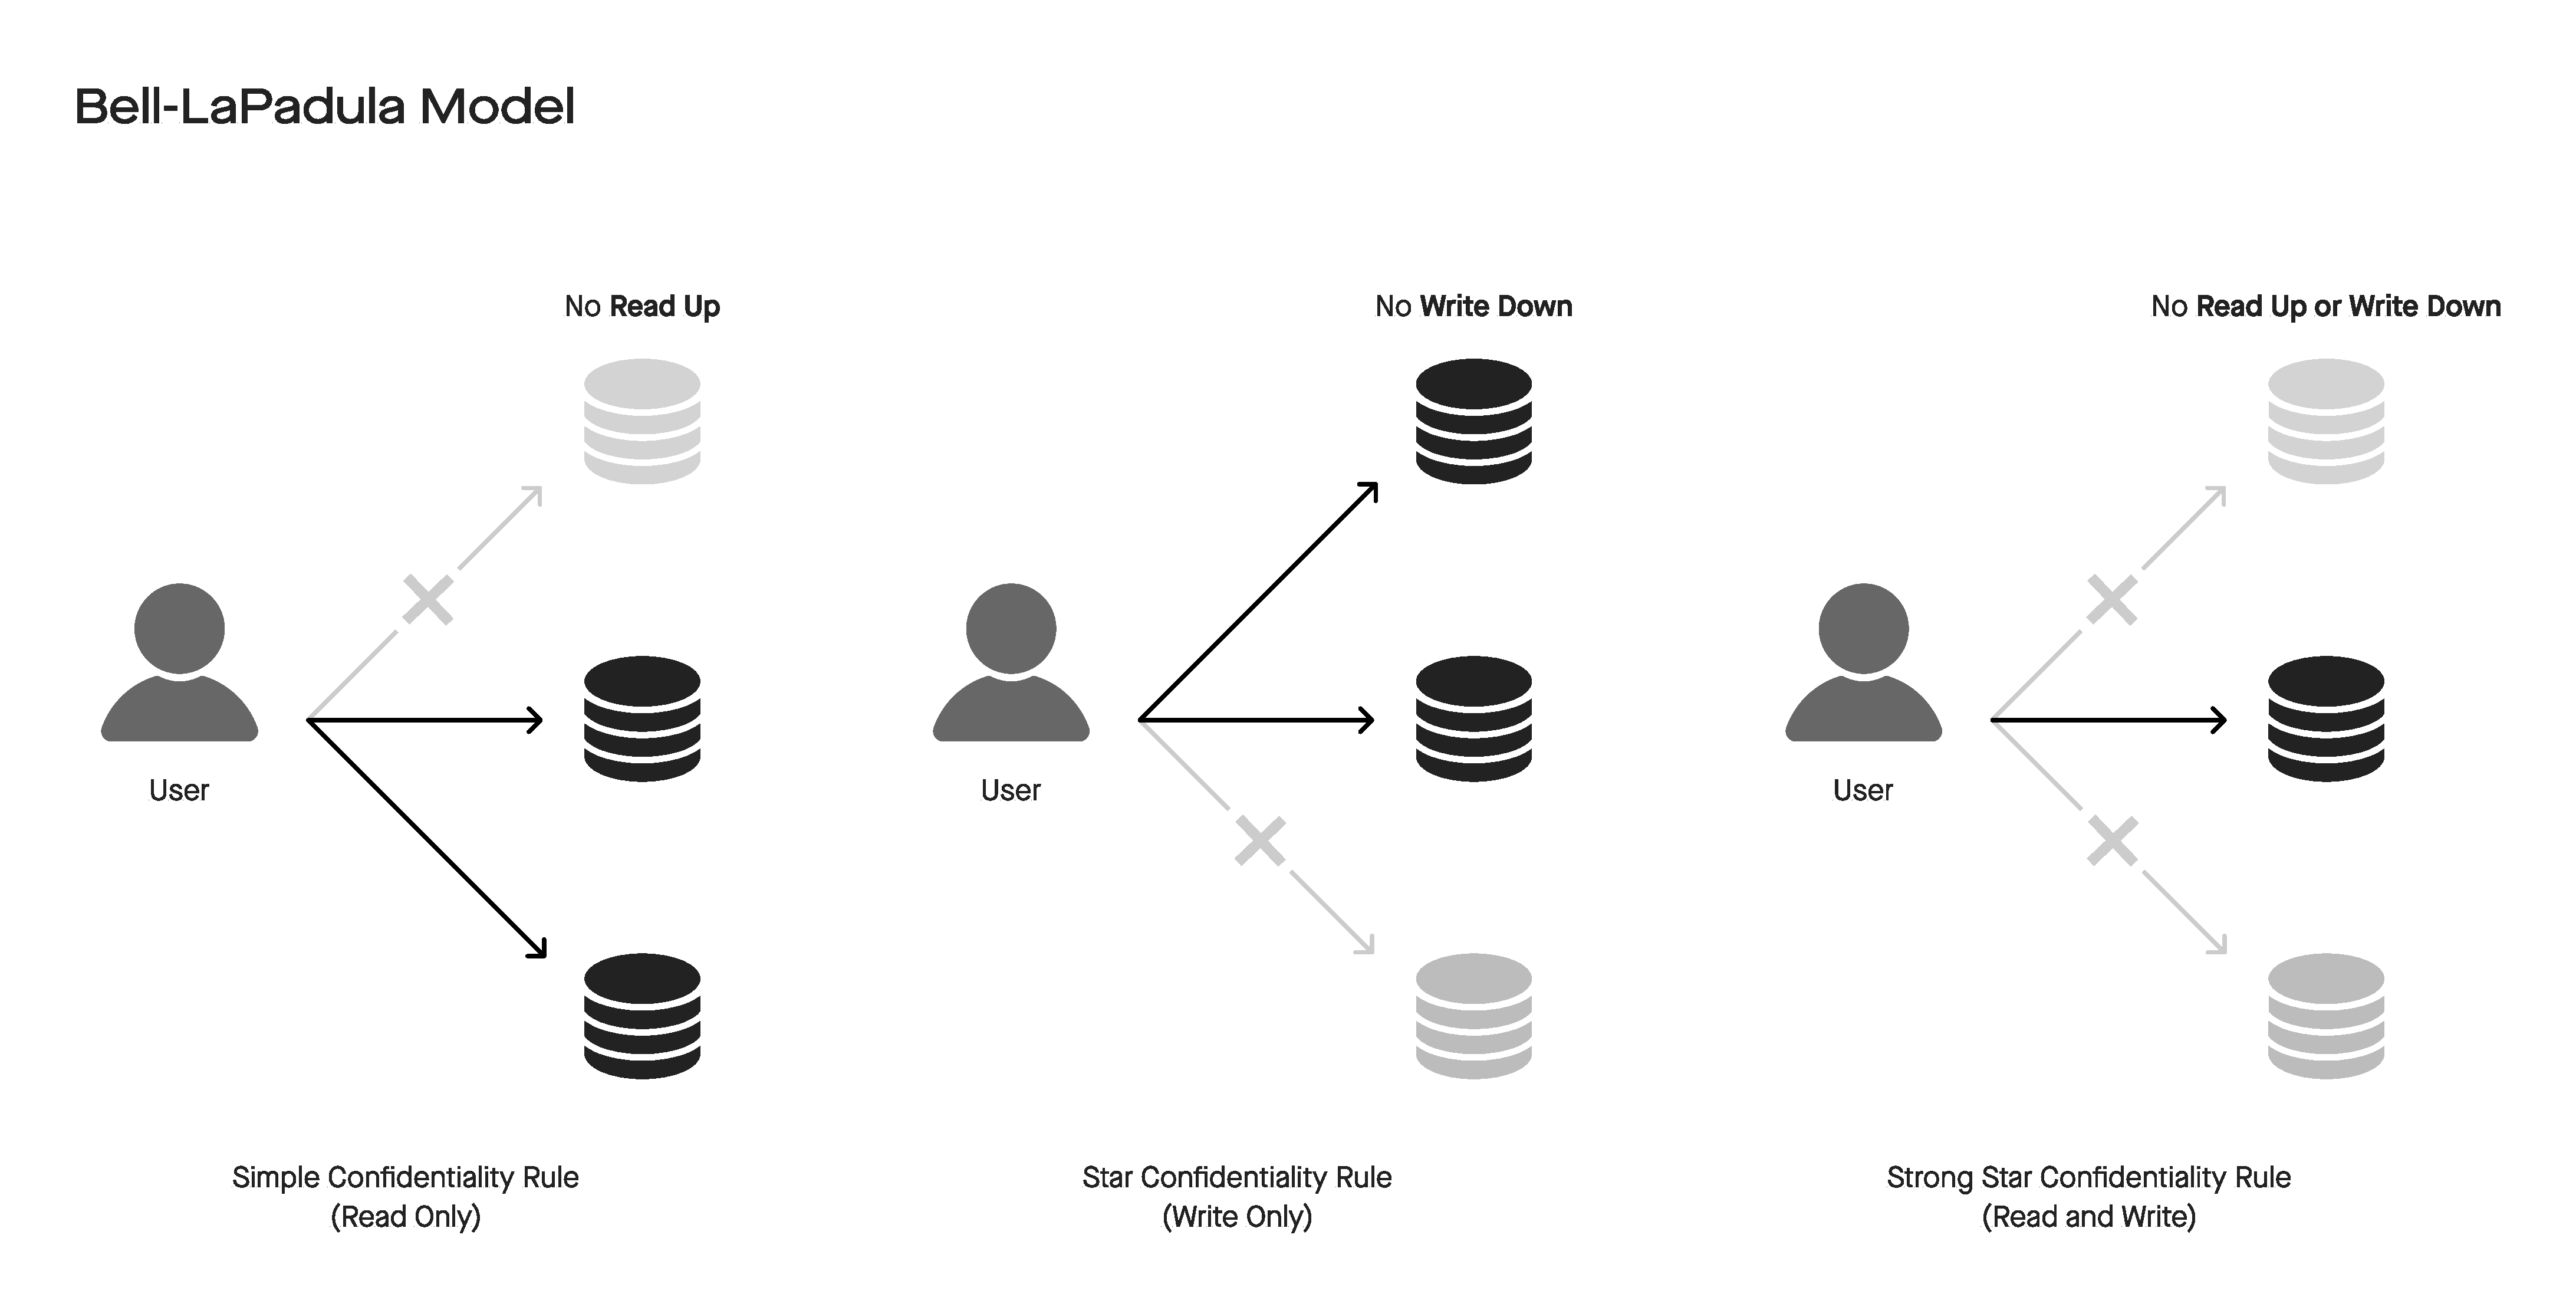
\includegraphics[clip, trim=0cm 2cm 0cm 6cm, width=0.80\textwidth]{./images/Bell-LaPadula_Model.pdf}
	}
	\caption{Bell-LaPadula Confidentiality Model}
	\label{fig: bella}
\end{figure*}


The appreciate ecosystem has blockchain gateway services that provide additional integrity. These services reside at the boundary of the appreciate ecosystem and facilitate communication between the platform and blockchains. Due to the rapid pace of evolution in blockchain technology, we have elected to keep this coupling loose and contained. This provides flexibility and extensibility in our integrated service offerings by decoupling our dependency from any single blockchain solution.

The specifics required for interoperability with a given blockchain are constrained to a small set of services responsible for communicating between the networks. Following open-source principles and community development, external entities can contribute components or knowledge to construct these gateways for many blockchains, including private ones. 


%\newpage

For instance, when a PoP Credential is associated with a high-value Item, we may issue a digital twin as an Item Token\cite{nfts}. The Item Owner may wish to transfer or replicate this token onto a different blockchain for a specific experience. Given that the PoP Credential acts as the record locator and source of truth, the accuracy of the system retains its integrity despite these reflections to external sources of truth.



\subsection{appreciate Ecosystem}

The appreciate ecosystem allows organizations to interact with Owners in a wide variety of ways. This means developers from those organizations must have free choice between many possible entry points into our ecosystem. The system can issue verifiable credentials (VCs) compliant with W3C Specifications\cite{verifiablecred}. As the VC and decentralized identifier (DiD) spaces mature, we expect our ecosystem will grow increasingly supportive of additional desired features.

Crucially, we are able to provide the same level of functionality and security regardless of which configuration our service providers choose to use -- whether they prefer a fully hosted “AWS Lambda"-style managed environment, the ability to deploy a Docker image\cite{modernapparch} to a managed environment similar to Kubernetes, 
or via one of a number of supplied example integration schemes. Examples would take the form of a Cryptogram-to-API bridge, Cryptogram-to-Kafka bridge, or a reverse-proxying service that could be run inside a VPC with no ingress.

To further offload work from development teams, we are also pleased to be able to offer our appreciate service library — home to a variety of data sources and downstream integrations that can be used out-of-the-box.

Additionally, the appreciate ecosystem’s health and status monitors allow companies to access insights into how an integration is performing and assess whether they are taking advantage of all the data and features available to them. They will also receive alerts when alterations to service interfaces are planned.


For appreciate’s initial set of service providers, see Appendix.~\ref{app: name}. 
For a diagram covering the high level architecture,  see \(Fig.~\ref{fig: app_plat} \). 

\begin{figure*}[!htb]
	\centering %trim=left botm right top
	%\fbox{
		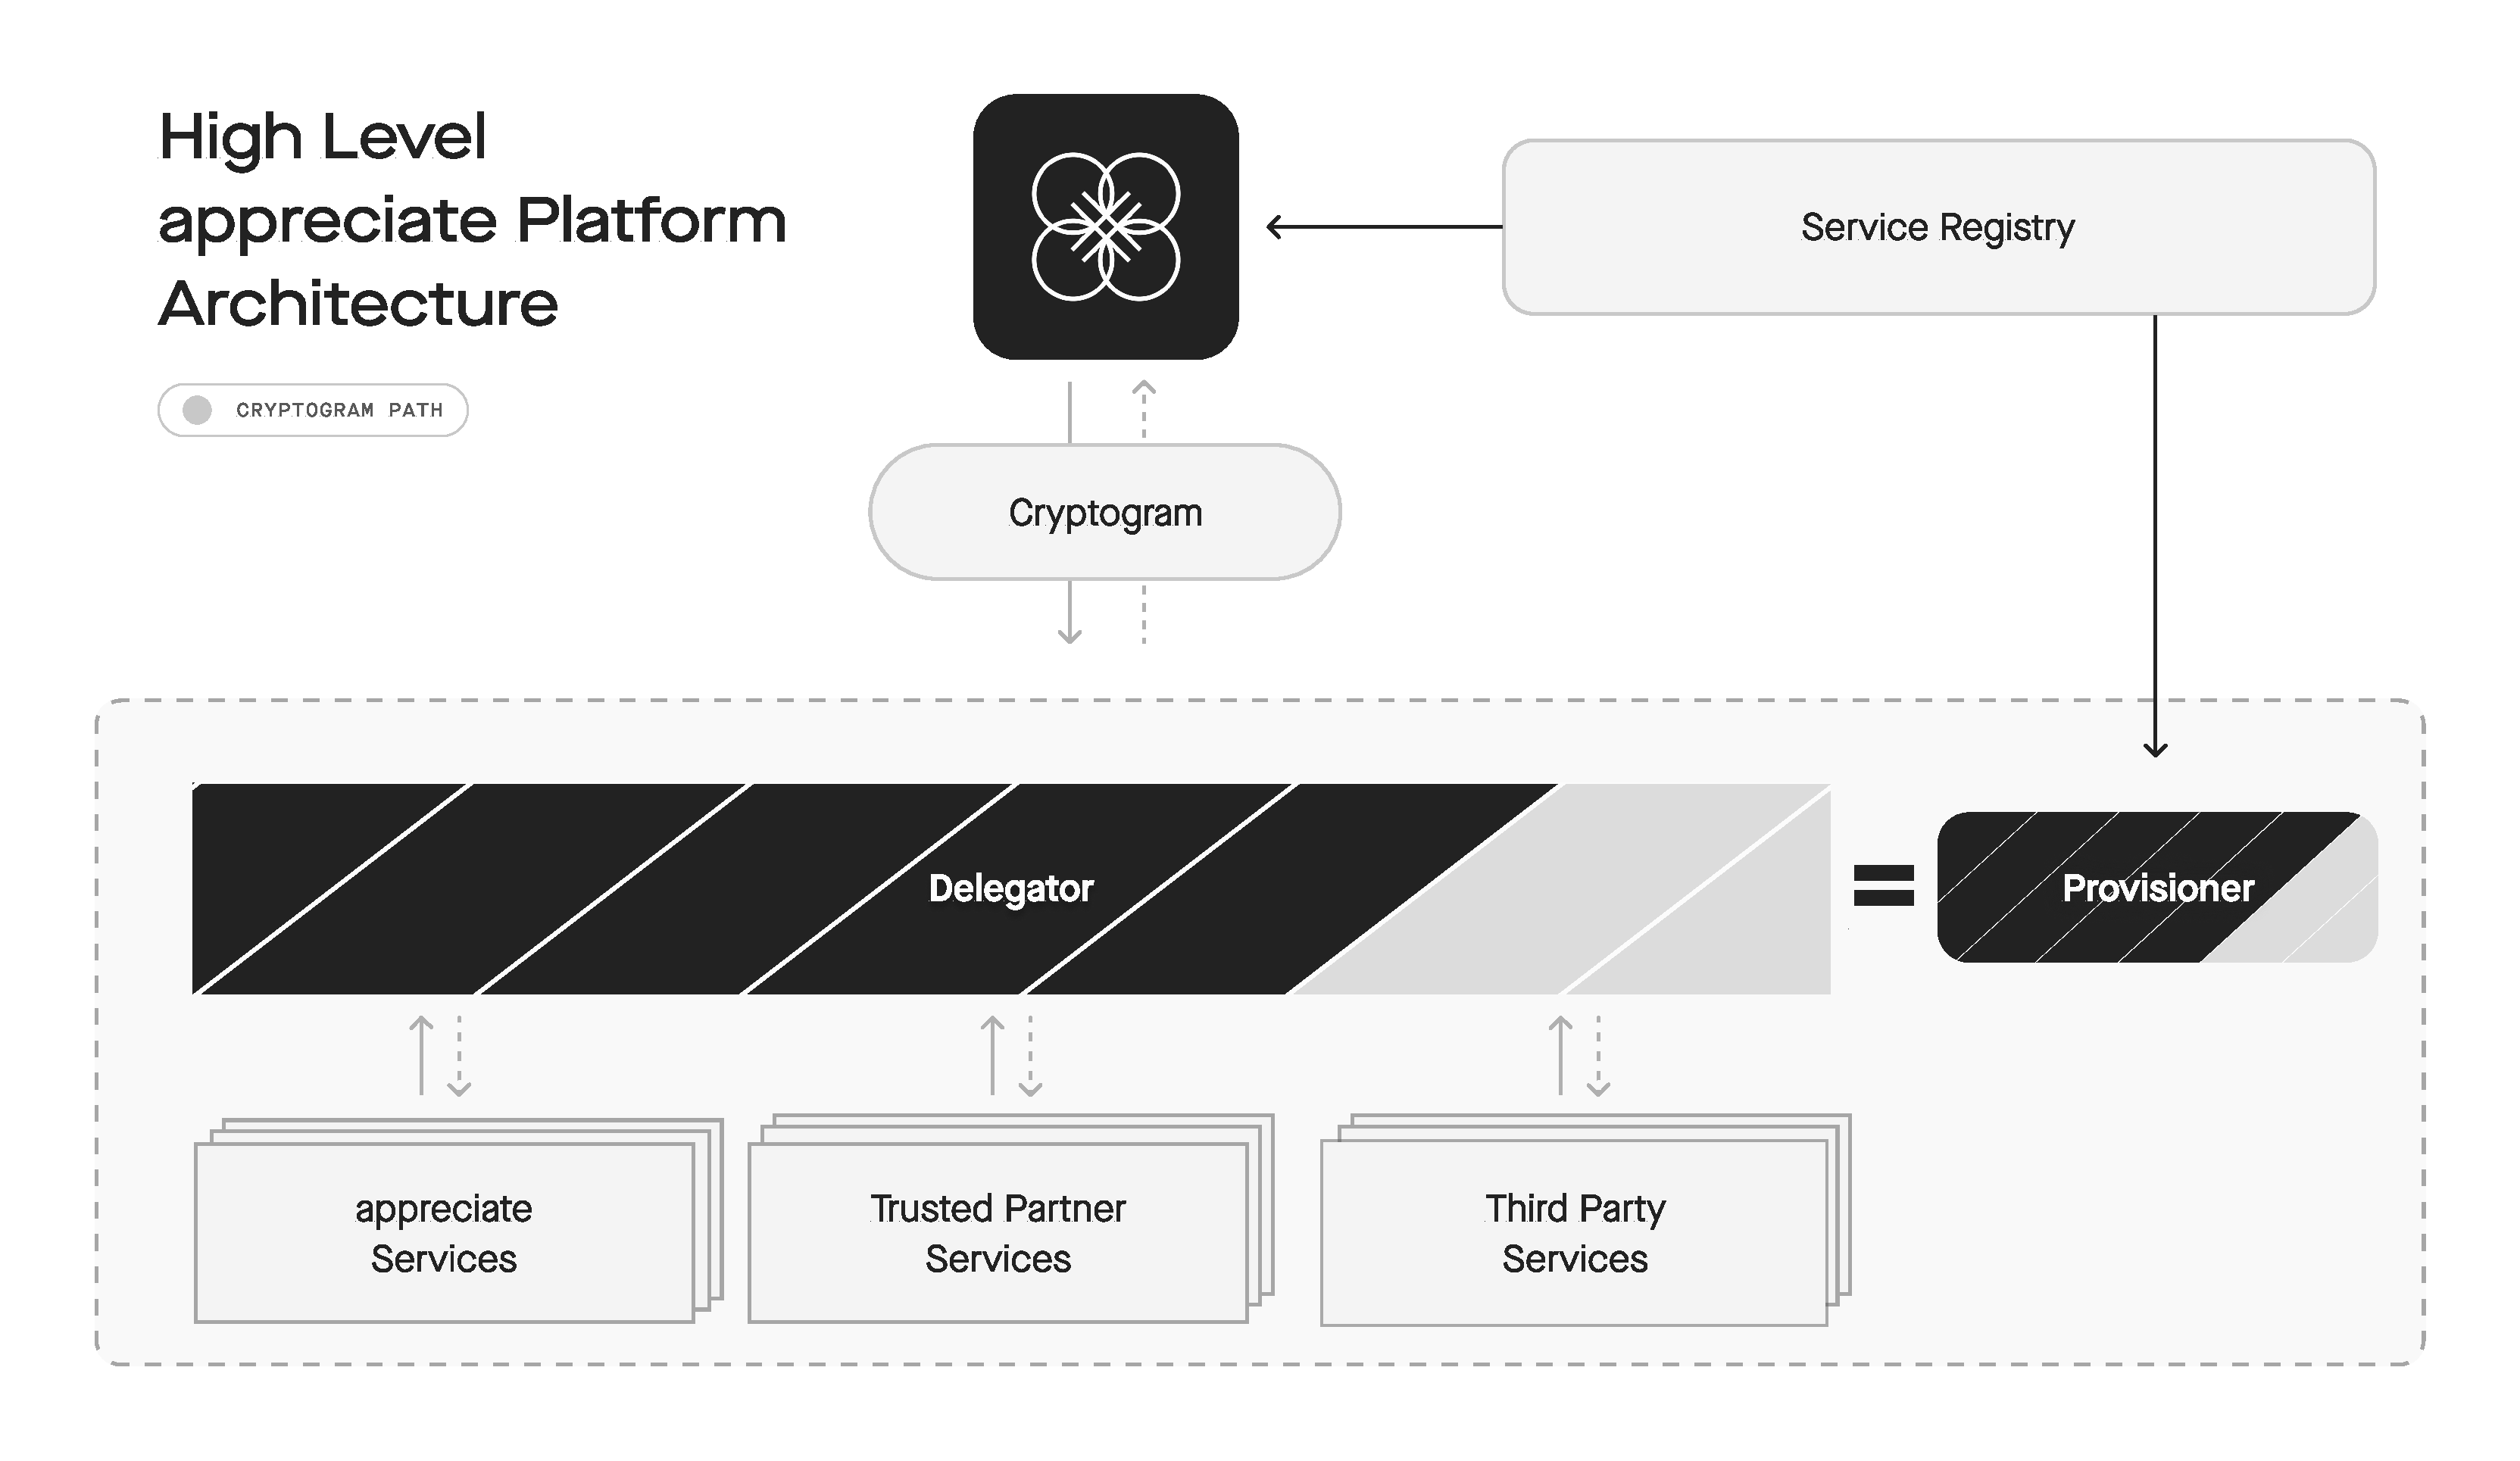
\includegraphics[clip, trim=0cm 2cm 0cm 2cm, width=0.80\textwidth]{./images/Architecture.pdf}
		%}
	\caption{Appreciate Platform Architecture}
	\label{fig: app_plat}
\end{figure*}

\subsection{Cryptograms}
A Cryptogram is a stateful, secure, routable structure that enables end-to-end encrypted communication throughout the appreciate ecosystem. Data is encrypted at the source, passed through the system, and decrypted on-demand by those entities with the appropriate keys. Following the principle of least privilege, decryption is handled for each service by a sidecar which is supplied with only the necessary decryption keys defined by the Service Registry.

Cryptograms allow for mediation between Owners and service providers, while maintaining data sovereignty for both parties.This means that the system, by design, can support services that manage their own encryption. In all cases, the Service Registry shares public keys for encryption. In the typical workflow, the system seeds the appropriate private keys onto a sidecar during service instantiation. Optionally, to support more secure communication to a service, the service owner may supply their own private key in the service logic by encapsulating it in the system image. An Integration API allows external service providers to register, submit, and update an application image and its keys for their implemented service (See \(Fig.~\ref{fig: infraint}\)).

\begin{figure*}[!htb]
	\centering %trim=left botm right top
	%\fbox{
		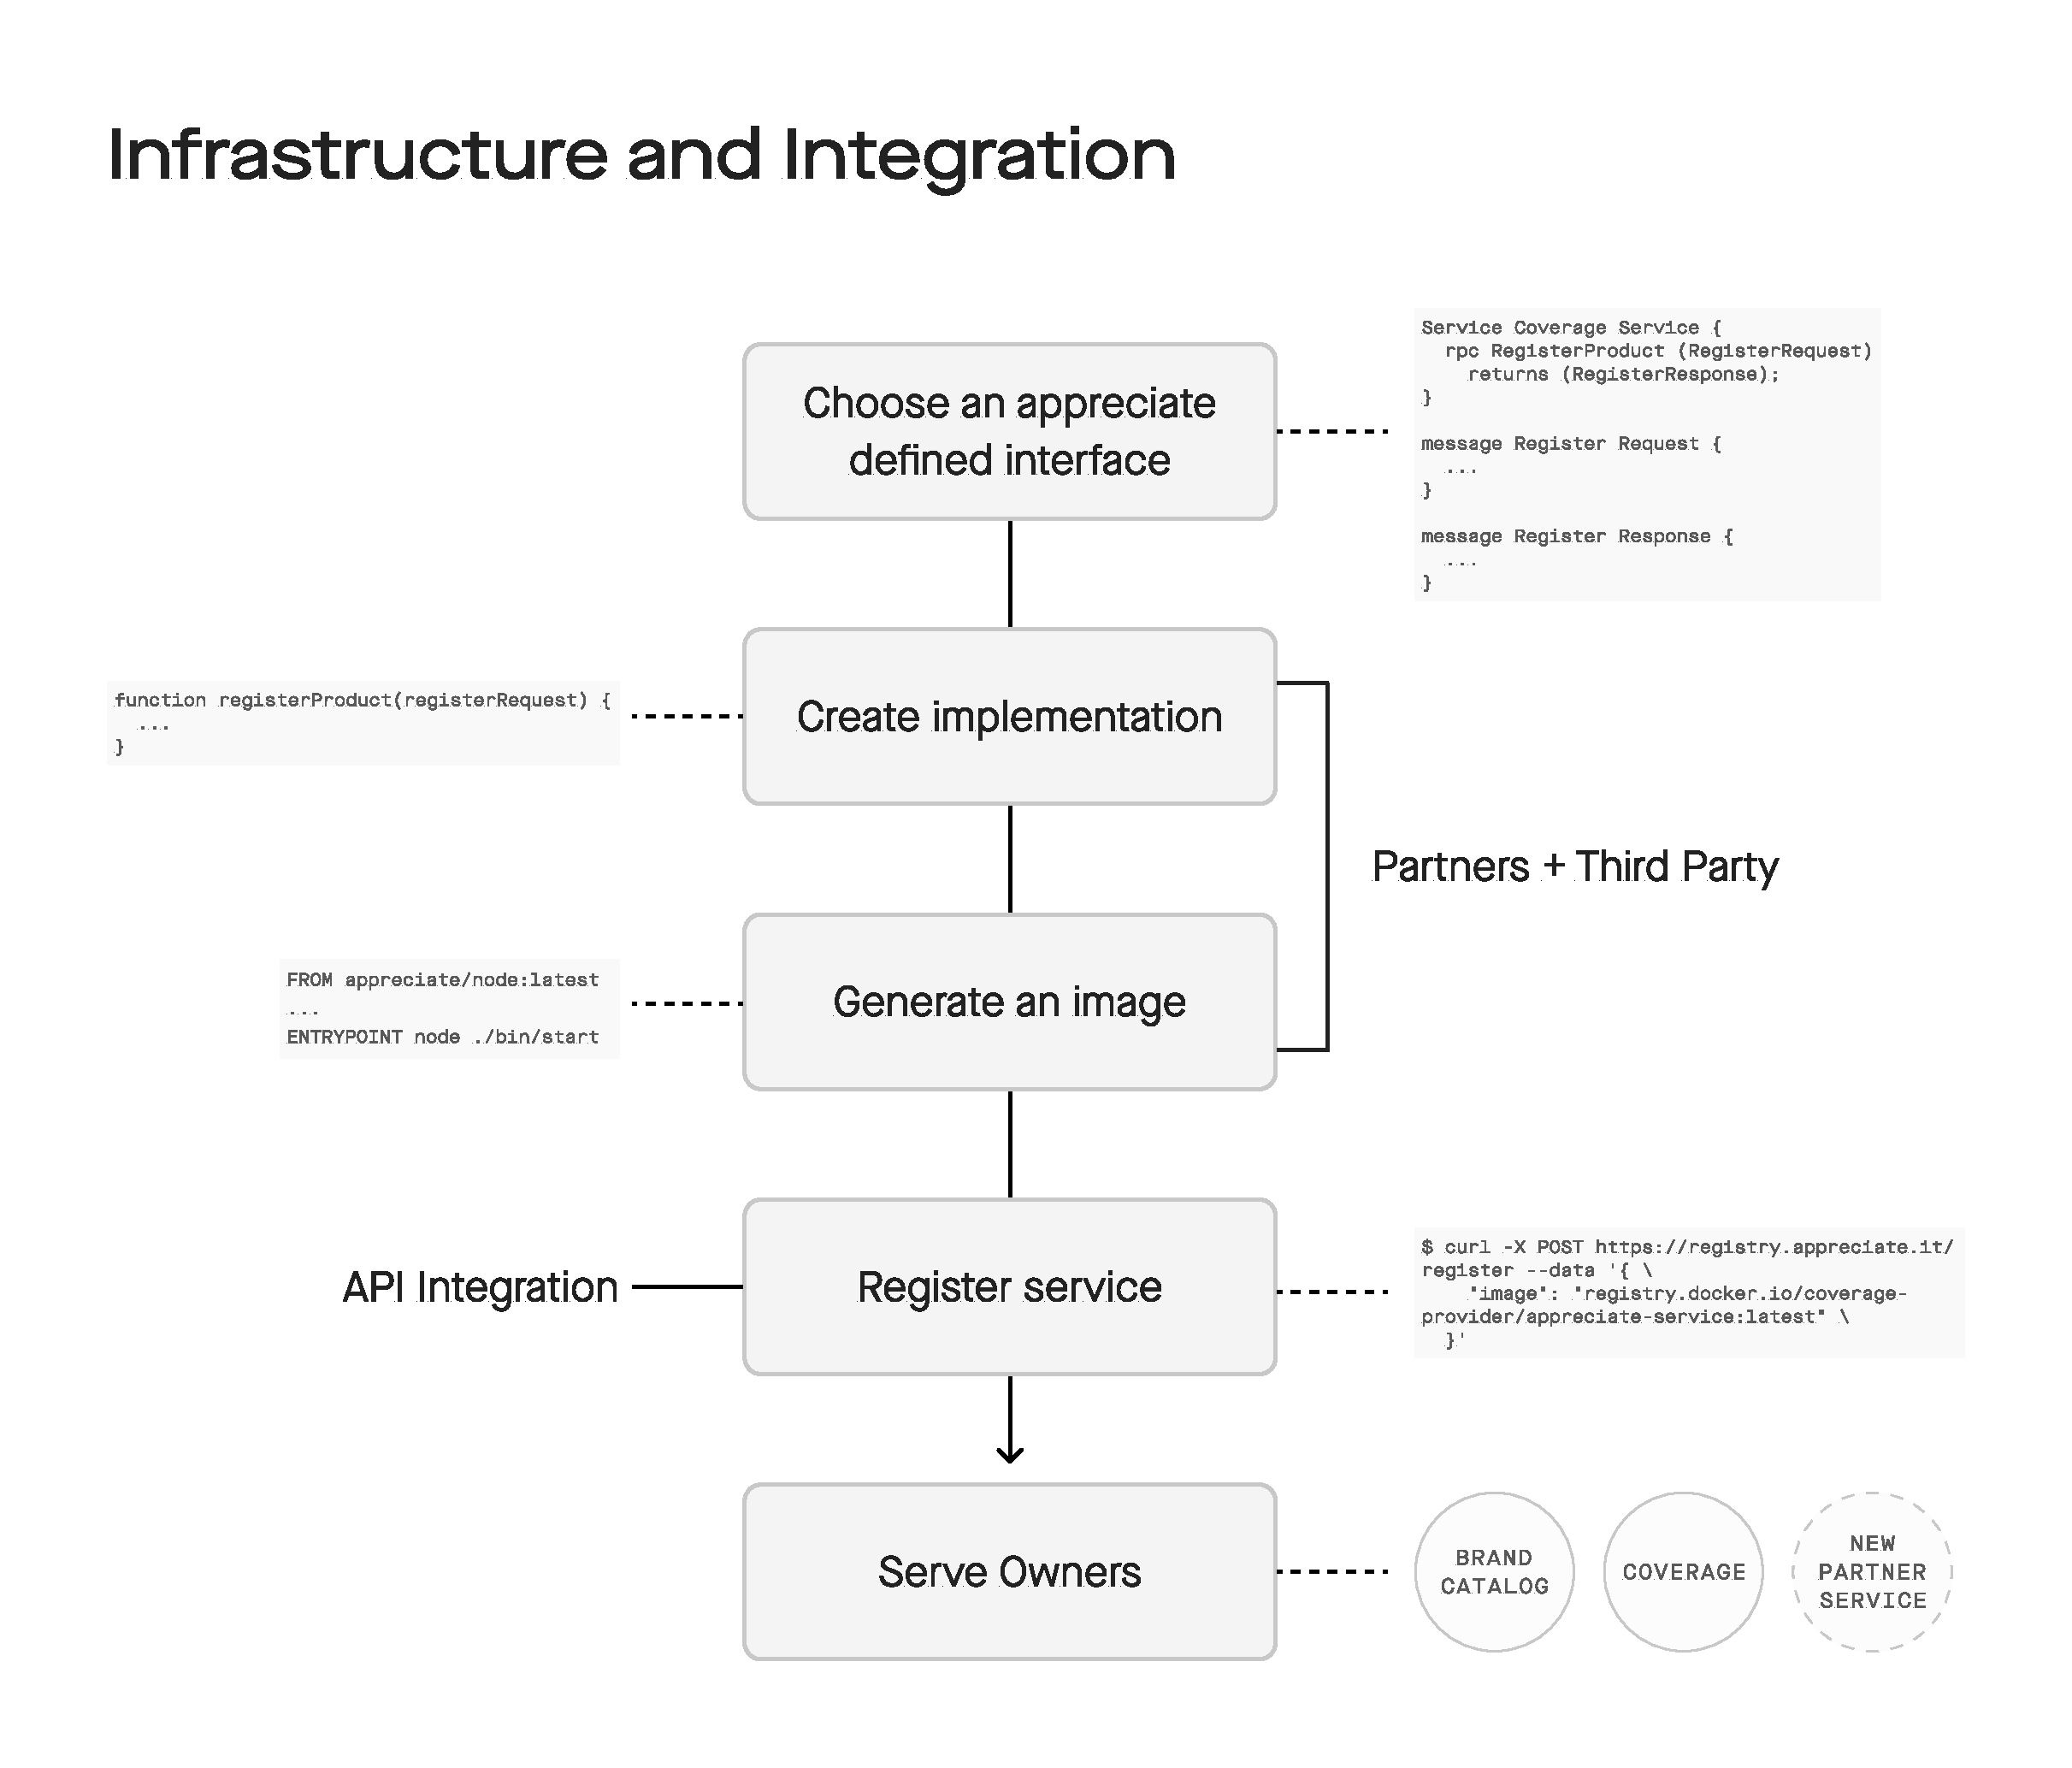
\includegraphics[clip, trim=0cm 2cm 0cm 5cm, width=0.80\textwidth]{./images/Infrasctructure_and_integration.pdf}
		%}
	\caption{Infrastructure and Integration}
	\label{fig: infraint}
\end{figure*}


A Cryptogram is created with a sequence of services that the Owner intends to leverage, as well as with the data required by those services. Both the Cryptogram’s list of services and the data components are encrypted for their intended recipients (e.g., a service, the system’s control plane, or the client).

The Cryptogram protocol enforces additive-only modifications, requiring all insertions to be signed by the originator -- creating a verifiable chain of custody and provable data integrity. This approach ensures that any service consuming the data can verify the origin and encrypt the response for the requestor. The appreciate ecosystem maintains its own key pairs to ensure that meta information, like routing, remains secure.


\subsection{Service Registry}

The Service Registry contains the definition and mapping of interfaces to concrete service implementations. Multiple services may exist for the same interface. Cryptograms may request either a specific service (implementation) of an interface or simply request ANY service that implements that interface, at which point the system will choose an appropriate service for the client.

An associated Key Vault, an independent system responsible for managing keys within the appreciate ecosystem, contains encrypted copies of the deployment keys for the registered services to enable them to bootstrap without leaking sensitive data. The Service Registry and associated Key Vault will be highly accessible as well as stored on-chain using a distributed filesystem (e.g. Ethereum with IPFS\cite{ipfs}).

\subsection{Provisioner}

The Provisioner is responsible for initializing services in the ecosystem. The Provisioner is paired 1:1 with a Delegator. When the Delegator requests an interface, the Provisioner will match it to an implementation in the Service Registry. The Provisioner will return an instance of the service to the Delegator.

The Provisioner maintains a pool of service instances (referred to here simply as “workers”) to enable the system to rapidly scale, meeting active Owners’ demand. All workers are initialized with an expiration date, after which they will be destroyed once they complete any outstanding tasks.

By queuing workers rather than data, the system not only side-steps the issues inherent in handling data-at-rest — like persistence, compliance, and consistency — it also allows the worker pool to “right size” itself through provisioning on-demand and self-destructing on disuse. Additionally, this forced expiry of service workers ensures the active worker pool is relatively fresh with any updated logic, keys, or configurations. 

\subsection{Delegator}
The Delegator controls routing in the appreciate ecosystem. This involves evaluating all incoming Cryptograms, decrypting the routing section, annotating state, and fetching the requested interfaces from the Provisioner.

The Delegator will request an instance of the desired service from the Provisioner and pass the Cryptogram to it. Once a service completes the processing of a Cryptogram, it returns the modified-and-signed Cryptogram to the Delegator for further routing to additional services or for returning to the requesting client. To provide some measure of idempotency without managing state itself, the Delegator may update the client with progress after receiving a response from a service with side-effects.


\subsection{Services}
In this system, a “service” is an executable implementation of a particular interface which is launched by the Provisioner. Services can be defined in a number of ways including Lambdas, Docker images, machine images, or build instructions.

Upon registration in the Service Registry, services are built and tested before being transformed into an appreciate service image. The appreciate service image is an accurate build of the service serialized in an input-ready state. This allows the Provisioner to instantiate services on-demand without incurring long build-times or provisioning overhead.

All service instances are instantiated with a configurable Time-To-Live (TTL), indicating its total service lifetime. Additionally, upon completion of work, the service registers its availability with the Provisioner to improve responsiveness by eliminating bootstrap times during high-demand periods. To further control fleet size, services set another TTL when entering the service queue and self-destruct after a period of time in the queue without action. These controls allow service worker pools to maintain a balance between responsiveness and resource management.

Services operate at different privilege levels. Following the principle of least privilege, the services owned by appreciate are restricted to the minimal level of access necessary to operate. Trusted partner services are audited to ensure they are also operating at the minimal level of access necessary. Untrusted, Third-Party Services are deployed into a limited-access sandbox, with network access restricted to a limited set of Cryptogram sidecar functionalities and the Delegator, as well as constraints on execution time and CPU/Memory usage.

The \textbf{Appendix A} lists the initial set of ownership service interfaces.

\section{Future Applications}

appreciate’s Extensible Ownership enables optimal Owner outcomes. By providing validated Proof of Ownership, appreciate facilitates seamless integration of third-party services, thus, lowering the economic barriers to entry (e.g. insurance only existed for high-value Items like engagement rings or luxury watches). Owners are empowered to access the services how they want, when they want, and for the price they want. Our PoP Credentials, M Score, and ecosystem enable third parties to transact with higher confidence in personhood and Item accuracy. Future contemplated applications of our ecosystem include:

\textbf{Owner to Owner Marketplace} \hfill \break
Currently, peer-to-peer marketplaces lack secure and trusted methods for exchanging Ownership and Items. The selling experience today is mired with lack of confidence in ownership, unknown Item quality, exchange and platform fees, and nefarious actors. appreciate offers a place for Owners to buy, sell, and exchange Items with endorsed Proof of Ownership - combining compliance, seamless procurement, and settlement. 

The appreciate marketplace and M Score informs risk to the future Owner, thus reducing the probability of purchasing fraudulent or defective Items. Additionally, exchange fees and settlement times are reduced as a result of not requiring human or third-party intermediaries in the transaction process. The Owner marketplace fosters a secure and trusted way of exchanging Items within an industry.


\textbf{Item Tracking As a Service} \hfill \break
Accuracy and Ownership of inventory movement through the supply chain is an issue that plagues all industries, old and new. Service providers can now identify the history of all Item data coming in and out of their supply chain. Item Tracking as a service grants the ability to control and manage increasingly complicated networks of manufacturers and suppliers when transparency, speed, agility, quality, and safety are critical. appreciate’s Item Tracking allows for increased precision in datasets and learning models enabling on-demand forecasting for inventory optimization, fulfillment, and reordering.

\textbf{Service Loyalty \& Rewards} \hfill \break
Currently, an Item’s history terminates after the point of sale. Critical insights like Ownership, chain-of-custody, Item modification, and Owner affinity are unidirectional and not visible to the original Item Issuer. By allowing bidirectional information exchange between Services and Owners, appreciate enables an opportunity for buyback programs, tailored services, and optimizing market availability by preference. Additionally, Owners can earn rewards (e.g. Tokens, discounts, special invitations, etc.). Vendors can create highly customized white-glove experiences encouraging Owner retention, brand loyalty, and long term engagement. 

\textbf{appreciate Tokens} \hfill \break
appreciate Tokens are generated to Owners based on Item affinity, participation, loyalty, etc. Tokens can be used towards future purchases and services made within the appreciate ecosystem. Increasing customer engagement, and strengthening the Owner relationship between the appreciate ecosystem and third party services.

\textbf{Dynamic NFTs (dNFT’s)} \hfill \break
Currently most NFTs are static and are immutable with fixed metadata. By issuing Dynamic NFT’s (dNFT’s), appreciate creates Items that retain their unique identifiers while updating aspects of their metadata based on trusted off-chain data sources and services. These Items are minted on-chain using hybrid smart contracts to access services within the appreciate ecosystem keeping the dNFTs metadata refreshed. Item Tokens representing real-world assets and M Scores require input where data can be refreshed. Additionally, Item attributes like customizations, damages or repair, history, and market value may be impacted over time. Owners have the opportunity to receive special access and rewards based on their dNFT status. 


\section{Conclusion}
appreciate is building the Owner Economy.  Our ecosystem is the optimal framework for Extensible Ownership - enabling Owners to do stuff with their stuff. Owners firmly control their data, digitally claim possession of their Items, and access a rich collection of service integrations. appreciate modernizes ownership in a way that is human meaningful, unifies physical and digital, all with unprecedented decentralization and security.

We are excited to explore the ecosystem’s potential; and ultimately, make a positive impact  for our Owners, our partners, and the planet...  Also, fuck receipts



\newpage
\appendix
\section{Services Appendix} \label{app: name}
 \renewcommand*{\arraystretch}{1.4}
	\begin{tabular}{|p{0.27\textwidth}|p{0.63\textwidth}|}			
	\hline
	\textbf{Ownership Services} & \textbf{Description}\\
	\hline 
	Pricing Services   & Owners can save, track, and monitor trends of Items  \\
	\hline
	Insurance & Owners can request and obtain approval to insure Items.  
		Based on Item verification and appraisals, appreciate can speed up the adjudication process for customers to receive insurance on their Items\\
		\hline
		Financial Services \& Credit & Owners can access credit based on the value of their Items \\
		\hline
		Repair & Owners can spend less time searching for repair services and improve the longevity of the Items they own \\
		\hline
		Marketplace &
		Owners can access a secondary marketplace of verified Items which they can buy, sell, and trade in a trusted manner. Sellers can make sales more quickly, and buyers enjoy a reduced risk of purchasing counterfeit goods. \\
		\hline
		VAT & Owners can request VAT back on Items purchased outside of their taxable home country, reducing the time they spend processing VAT and receiving a refund \\
		\hline
		Verifiable Credentials (VCs) &
		Items can have verifiable credentials (VCs) issued and verified for different attestations regarding associated details.  \\
		\hline
		Blockchain Services &
		Blockchain gateway services support interoperability with blockchains (e.g. Ethereum).
		A transaction signer with elevated security will enable approval of custodial wallet transactions.
		Some of the supported blockchains also will include services to monitor transactions (potentially enable recovery for a stuck transaction)
		Additionally, a distributed file system gateway supports interoperability with distributed file systems, including support for long-term persistence (e.g., IPFS with Infura)
		NFT managers mint and verify NFTs on specific blockchains(i.e. mint Ethereum non-fungible tokens (NFT)\cite{eth1155})\\
		\hline
\end{tabular}



\newpage
\begin{thebibliography}{9}
	 
	\bibitem{envimp}
	Environmental Impact of Receipts https://www.greenamerica.org/sites/default/files/2019-06/Green America’s Skip The Slip Report.pdf 
	
	\bibitem{zooko}
	Bob Wyman, “The Persistence of Identity (Updating Zooko's Pyramid)” \_As I May Think…\_ 30 Dec 2016. \url{https://web.archive.org/web/20160331154849/https://wyman.us/main/2006/12/the_persistence.html}	
	
	\bibitem{biba}
	Biba, K. J. "Integrity Considerations for Secure Computer Systems", MTR-3153, The Mitre Corporation, June 1975.
	
	\bibitem{securecomp}
	Bell, David Elliott \& LaPadula, Leonard J. (1973). "Secure Computer Systems: Mathematical Foundations" (PDF). MITRE Corporation. Archived from the original (PDF) on 2006-06-18. Retrieved 2006-04-20.
	
	\bibitem{nfts}
	Redeem-and-retain NFTs are the future of luxury goods (2022, July 27). Nic Carter
	\url{https://medium.com/@nic__carter/redeem-and-retain-nfts-are-the-future-of-luxury-goods-760f00dbce23}

	\bibitem{verifiablecred}
	Verifiable Credentials Data Model(VC) https://www.w3.org/TR/2022/REC-vc-data-model-20220303/

	\bibitem{modernapparch}
	Modern App Architecture for the Enterprise \\
	\url{https://www.docker.com/wp-content/uploads/2022/03/caaSwhitepaper_V6_0.pdf}

	\bibitem{eth1155}
	Ethereum ERC-1155 Multi-Token Standard \\ \url{https://ethereum.org/en/developers/docs/standards/tokens/erc-1155/}

	\bibitem{ipfs}
   IPFS, \url{https://docs.ipfs.tech/concepts/what-is-ipfs/#decentralization}
	

	
\end{thebibliography}
	
\end{document}
